\documentclass[twoside]{book}

% Packages required by doxygen
\usepackage{fixltx2e}
\usepackage{calc}
\usepackage{doxygen}
\usepackage[export]{adjustbox} % also loads graphicx
\usepackage{graphicx}
\usepackage[utf8]{inputenc}
\usepackage{makeidx}
\usepackage{multicol}
\usepackage{multirow}
\PassOptionsToPackage{warn}{textcomp}
\usepackage{textcomp}
\usepackage[nointegrals]{wasysym}
\usepackage[table]{xcolor}

% NLS support packages
\usepackage[french]{babel}

% Font selection
\usepackage[T1]{fontenc}
\usepackage[scaled=.90]{helvet}
\usepackage{courier}
\usepackage{amssymb}
\usepackage{sectsty}
\renewcommand{\familydefault}{\sfdefault}
\allsectionsfont{%
  \fontseries{bc}\selectfont%
  \color{darkgray}%
}
\renewcommand{\DoxyLabelFont}{%
  \fontseries{bc}\selectfont%
  \color{darkgray}%
}
\newcommand{\+}{\discretionary{\mbox{\scriptsize$\hookleftarrow$}}{}{}}

% Page & text layout
\usepackage{geometry}
\geometry{%
  a4paper,%
  top=2.5cm,%
  bottom=2.5cm,%
  left=2.5cm,%
  right=2.5cm%
}
\tolerance=750
\hfuzz=15pt
\hbadness=750
\setlength{\emergencystretch}{15pt}
\setlength{\parindent}{0cm}
\setlength{\parskip}{0.2cm}
\makeatletter
\renewcommand{\paragraph}{%
  \@startsection{paragraph}{4}{0ex}{-1.0ex}{1.0ex}{%
    \normalfont\normalsize\bfseries\SS@parafont%
  }%
}
\renewcommand{\subparagraph}{%
  \@startsection{subparagraph}{5}{0ex}{-1.0ex}{1.0ex}{%
    \normalfont\normalsize\bfseries\SS@subparafont%
  }%
}
\makeatother

% Headers & footers
\usepackage{fancyhdr}
\pagestyle{fancyplain}
\fancyhead[LE]{\fancyplain{}{\bfseries\thepage}}
\fancyhead[CE]{\fancyplain{}{}}
\fancyhead[RE]{\fancyplain{}{\bfseries\leftmark}}
\fancyhead[LO]{\fancyplain{}{\bfseries\rightmark}}
\fancyhead[CO]{\fancyplain{}{}}
\fancyhead[RO]{\fancyplain{}{\bfseries\thepage}}
\fancyfoot[LE]{\fancyplain{}{}}
\fancyfoot[CE]{\fancyplain{}{}}
\fancyfoot[RE]{\fancyplain{}{\bfseries\scriptsize Généré le Lundi 23 Novembre 2015 21\+:43\+:02 pour Ruzzle Solver par Doxygen }}
\fancyfoot[LO]{\fancyplain{}{\bfseries\scriptsize Généré le Lundi 23 Novembre 2015 21\+:43\+:02 pour Ruzzle Solver par Doxygen }}
\fancyfoot[CO]{\fancyplain{}{}}
\fancyfoot[RO]{\fancyplain{}{}}
\renewcommand{\footrulewidth}{0.4pt}
\renewcommand{\chaptermark}[1]{%
  \markboth{#1}{}%
}
\renewcommand{\sectionmark}[1]{%
  \markright{\thesection\ #1}%
}

% Indices & bibliography
\usepackage{natbib}
\usepackage[titles]{tocloft}
\setcounter{tocdepth}{3}
\setcounter{secnumdepth}{5}
\makeindex

% Hyperlinks (required, but should be loaded last)
\usepackage{ifpdf}
\ifpdf
  \usepackage[pdftex,pagebackref=true]{hyperref}
\else
  \usepackage[ps2pdf,pagebackref=true]{hyperref}
\fi
\hypersetup{%
  colorlinks=true,%
  linkcolor=blue,%
  citecolor=blue,%
  unicode%
}

% Custom commands
\newcommand{\clearemptydoublepage}{%
  \newpage{\pagestyle{empty}\cleardoublepage}%
}


%===== C O N T E N T S =====

\begin{document}

% Titlepage & ToC
\hypersetup{pageanchor=false,
             bookmarks=true,
             bookmarksnumbered=true,
             pdfencoding=unicode
            }
\pagenumbering{roman}
\begin{titlepage}
\vspace*{7cm}
\begin{center}%
{\Large Ruzzle Solver }\\
\vspace*{1cm}
{\large Généré par Doxygen 1.8.10}\\
\vspace*{0.5cm}
{\small Lundi 23 Novembre 2015 21:43:02}\\
\end{center}
\end{titlepage}
\clearemptydoublepage
\tableofcontents
\clearemptydoublepage
\pagenumbering{arabic}
\hypersetup{pageanchor=true}

%--- Begin generated contents ---
\chapter{Page principale}
\label{index}\hypertarget{index}{}Ce programme à été conçue dans le cadre d\textquotesingle{}un projet de seconde année de License S\+P\+I à l\textquotesingle{}Université du Maine -\/ Le Mans

Ce programme à pour but de résoudre une grille du jeux pour smartphone Ruzzle \+:



Il est possible d\textquotesingle{}utilisé ce programme soit \+:
\begin{DoxyItemize}
\item En C\+L\+I en passant dirrectement la chaine de caractère qui défini la grille \begin{DoxyVerb}  > ruzzle_solver "V5  R1  L2  S1  T1  N1  I1  V5  C3MTL2  A1  R1  D2  E1  S1  E1  "
\end{DoxyVerb}

\item En entrent la chaine de caractère lorsqu\textquotesingle{}elle est demandée.
\end{DoxyItemize}

Auteurs \+: Ewen C. -\/ Bastien 
\chapter{Index des structures de données}
\section{Structures de données}
Liste des structures de données avec une brève description \+:\begin{DoxyCompactList}
\item\contentsline{section}{\hyperlink{structcell}{cell} \\*Défini une case de la grille, l\textquotesingle{}élément \textquotesingle{}visited\textquotesingle{} est utilisé lors de la recherche de mot }{\pageref{db/d76/structcell}}{}
\item\contentsline{section}{\hyperlink{structcoord}{coord} \\*Défini des coordonnée d\textquotesingle{}une case de la grille }{\pageref{d6/dc6/structcoord}}{}
\item\contentsline{section}{\hyperlink{structelement}{element} \\*Structure de donnée formant un élément de la liste }{\pageref{d9/db2/structelement}}{}
\item\contentsline{section}{\hyperlink{structt__score}{t\+\_\+score} \\*Défini le score du mot que l\textquotesingle{}on est en train de chercher }{\pageref{d7/dfc/structt__score}}{}
\end{DoxyCompactList}

\chapter{Index des fichiers}
\section{Liste des fichiers}
Liste de tous les fichiers avec une brève description \+:\begin{DoxyCompactList}
\item\contentsline{section}{\hyperlink{liste_8c}{liste.\+c} \\*Programme de gestion d\textquotesingle{}une liste }{\pageref{d3/dc8/liste_8c}}{}
\item\contentsline{section}{\hyperlink{liste_8h}{liste.\+h} }{\pageref{d4/d5b/liste_8h}}{}
\item\contentsline{section}{\hyperlink{main_8c}{main.\+c} \\*Programme principal }{\pageref{d0/d29/main_8c}}{}
\item\contentsline{section}{\hyperlink{ruzzle_8c}{ruzzle.\+c} \\*Fonctions du ruzzle solver }{\pageref{d3/df5/ruzzle_8c}}{}
\item\contentsline{section}{\hyperlink{ruzzle_8h}{ruzzle.\+h} }{\pageref{df/d02/ruzzle_8h}}{}
\end{DoxyCompactList}

\chapter{Documentation des structures de données}
\hypertarget{structcell}{}\section{Référence de la structure cell}
\label{structcell}\index{cell@{cell}}


Défini une case de la grille, l\textquotesingle{}élément \textquotesingle{}visited\textquotesingle{} est utilisé lors de la recherche de mot.  




{\ttfamily \#include $<$ruzzle.\+h$>$}



Graphe de collaboration de cell\+:
\nopagebreak
\begin{figure}[H]
\begin{center}
\leavevmode
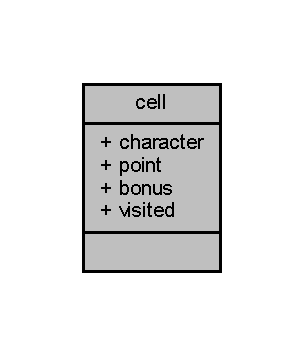
\includegraphics[width=146pt]{db/d45/structcell__coll__graph}
\end{center}
\end{figure}
\subsection*{Champs de données}
\begin{DoxyCompactItemize}
\item 
unsigned char \hyperlink{structcell_abe31bdd62e498dce604b14e75df142dd}{character}
\item 
unsigned int \hyperlink{structcell_a914cae0a595952eda16c33e4ca9c1cbb}{point}
\item 
\hyperlink{ruzzle_8h_af98046282a9e785a234a2ea7b10681f2}{bonus\+Enum} \hyperlink{structcell_a1724452b0364c62e84a310b3c29e80bc}{bonus}
\item 
unsigned int \hyperlink{structcell_ac5ab8c056a470676e0b6689ffdda1a05}{visited}
\end{DoxyCompactItemize}


\subsection{Description détaillée}
Défini une case de la grille, l\textquotesingle{}élément \textquotesingle{}visited\textquotesingle{} est utilisé lors de la recherche de mot. 

Définition à la ligne 23 du fichier ruzzle.\+h.



\subsection{Documentation des champs}
\hypertarget{structcell_a1724452b0364c62e84a310b3c29e80bc}{}\index{cell@{cell}!bonus@{bonus}}
\index{bonus@{bonus}!cell@{cell}}
\subsubsection[{bonus}]{\setlength{\rightskip}{0pt plus 5cm}{\bf bonus\+Enum} bonus}\label{structcell_a1724452b0364c62e84a310b3c29e80bc}


Définition à la ligne 27 du fichier ruzzle.\+h.

\hypertarget{structcell_abe31bdd62e498dce604b14e75df142dd}{}\index{cell@{cell}!character@{character}}
\index{character@{character}!cell@{cell}}
\subsubsection[{character}]{\setlength{\rightskip}{0pt plus 5cm}unsigned char character}\label{structcell_abe31bdd62e498dce604b14e75df142dd}


Définition à la ligne 25 du fichier ruzzle.\+h.

\hypertarget{structcell_a914cae0a595952eda16c33e4ca9c1cbb}{}\index{cell@{cell}!point@{point}}
\index{point@{point}!cell@{cell}}
\subsubsection[{point}]{\setlength{\rightskip}{0pt plus 5cm}unsigned int point}\label{structcell_a914cae0a595952eda16c33e4ca9c1cbb}


Définition à la ligne 26 du fichier ruzzle.\+h.

\hypertarget{structcell_ac5ab8c056a470676e0b6689ffdda1a05}{}\index{cell@{cell}!visited@{visited}}
\index{visited@{visited}!cell@{cell}}
\subsubsection[{visited}]{\setlength{\rightskip}{0pt plus 5cm}unsigned int visited}\label{structcell_ac5ab8c056a470676e0b6689ffdda1a05}


Définition à la ligne 28 du fichier ruzzle.\+h.



La documentation de cette structure a été générée à partir du fichier suivant \+:\begin{DoxyCompactItemize}
\item 
\hyperlink{ruzzle_8h}{ruzzle.\+h}\end{DoxyCompactItemize}

\hypertarget{structcoord}{}\section{Référence de la structure coord}
\label{structcoord}\index{coord@{coord}}


Défini des coordonnée d\textquotesingle{}une case de la grille.  




{\ttfamily \#include $<$ruzzle.\+h$>$}



Graphe de collaboration de coord\+:
\nopagebreak
\begin{figure}[H]
\begin{center}
\leavevmode
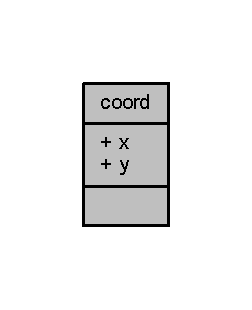
\includegraphics[width=121pt]{d9/d49/structcoord__coll__graph}
\end{center}
\end{figure}
\subsection*{Champs de données}
\begin{DoxyCompactItemize}
\item 
int \hyperlink{structcoord_a6150e0515f7202e2fb518f7206ed97dc}{x}
\item 
int \hyperlink{structcoord_a0a2f84ed7838f07779ae24c5a9086d33}{y}
\end{DoxyCompactItemize}


\subsection{Description détaillée}
Défini des coordonnée d\textquotesingle{}une case de la grille. 

Définition à la ligne 36 du fichier ruzzle.\+h.



\subsection{Documentation des champs}
\hypertarget{structcoord_a6150e0515f7202e2fb518f7206ed97dc}{}\index{coord@{coord}!x@{x}}
\index{x@{x}!coord@{coord}}
\subsubsection[{x}]{\setlength{\rightskip}{0pt plus 5cm}int x}\label{structcoord_a6150e0515f7202e2fb518f7206ed97dc}


Définition à la ligne 38 du fichier ruzzle.\+h.

\hypertarget{structcoord_a0a2f84ed7838f07779ae24c5a9086d33}{}\index{coord@{coord}!y@{y}}
\index{y@{y}!coord@{coord}}
\subsubsection[{y}]{\setlength{\rightskip}{0pt plus 5cm}int y}\label{structcoord_a0a2f84ed7838f07779ae24c5a9086d33}


Définition à la ligne 39 du fichier ruzzle.\+h.



La documentation de cette structure a été générée à partir du fichier suivant \+:\begin{DoxyCompactItemize}
\item 
\hyperlink{ruzzle_8h}{ruzzle.\+h}\end{DoxyCompactItemize}

\hypertarget{structelement}{}\section{Référence de la structure element}
\label{structelement}\index{element@{element}}


Structure de donnée formant un élément de la liste.  




Graphe de collaboration de element\+:
\nopagebreak
\begin{figure}[H]
\begin{center}
\leavevmode
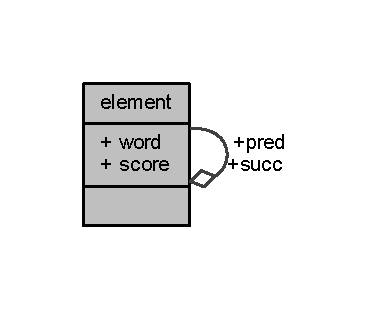
\includegraphics[width=177pt]{da/d80/structelement__coll__graph}
\end{center}
\end{figure}
\subsection*{Champs de données}
\begin{DoxyCompactItemize}
\item 
char \hyperlink{structelement_af034065dfe33f7ef74362e100b14b260}{word} \mbox{[}20\mbox{]}
\item 
int \hyperlink{structelement_aef160b7437d94056f1dc59646cd5b87d}{score}
\item 
struct \hyperlink{structelement}{element} $\ast$ \hyperlink{structelement_a932b74e6abe994b7316f4347a70d215b}{pred}
\item 
struct \hyperlink{structelement}{element} $\ast$ \hyperlink{structelement_a28a298bdc8522e913d39bf3f672ff5e5}{succ}
\end{DoxyCompactItemize}


\subsection{Description détaillée}
Structure de donnée formant un élément de la liste. 

Définition à la ligne 24 du fichier liste.\+c.



\subsection{Documentation des champs}
\hypertarget{structelement_a932b74e6abe994b7316f4347a70d215b}{}\index{element@{element}!pred@{pred}}
\index{pred@{pred}!element@{element}}
\subsubsection[{pred}]{\setlength{\rightskip}{0pt plus 5cm}struct {\bf element}$\ast$ pred}\label{structelement_a932b74e6abe994b7316f4347a70d215b}
Pointeur vers l\textquotesingle{}élément précedent 

Définition à la ligne 28 du fichier liste.\+c.

\hypertarget{structelement_aef160b7437d94056f1dc59646cd5b87d}{}\index{element@{element}!score@{score}}
\index{score@{score}!element@{element}}
\subsubsection[{score}]{\setlength{\rightskip}{0pt plus 5cm}int score}\label{structelement_aef160b7437d94056f1dc59646cd5b87d}
Score enregistré dans l\textquotesingle{}élément de la chaine 

Définition à la ligne 27 du fichier liste.\+c.

\hypertarget{structelement_a28a298bdc8522e913d39bf3f672ff5e5}{}\index{element@{element}!succ@{succ}}
\index{succ@{succ}!element@{element}}
\subsubsection[{succ}]{\setlength{\rightskip}{0pt plus 5cm}struct {\bf element}$\ast$ succ}\label{structelement_a28a298bdc8522e913d39bf3f672ff5e5}
Pointeur vers l\textquotesingle{}élément suivant 

Définition à la ligne 29 du fichier liste.\+c.

\hypertarget{structelement_af034065dfe33f7ef74362e100b14b260}{}\index{element@{element}!word@{word}}
\index{word@{word}!element@{element}}
\subsubsection[{word}]{\setlength{\rightskip}{0pt plus 5cm}char word\mbox{[}20\mbox{]}}\label{structelement_af034065dfe33f7ef74362e100b14b260}
Chaine de caractère enregistré dans l\textquotesingle{}élément de la chaine 

Définition à la ligne 26 du fichier liste.\+c.



La documentation de cette structure a été générée à partir du fichier suivant \+:\begin{DoxyCompactItemize}
\item 
\hyperlink{liste_8c}{liste.\+c}\end{DoxyCompactItemize}

\hypertarget{structt__score}{}\section{Référence de la structure t\+\_\+score}
\label{structt__score}\index{t\+\_\+score@{t\+\_\+score}}


défini le score du mot que l\textquotesingle{}on est en train de chercher.  




{\ttfamily \#include $<$ruzzle.\+h$>$}



Graphe de collaboration de t\+\_\+score\+:
\nopagebreak
\begin{figure}[H]
\begin{center}
\leavevmode
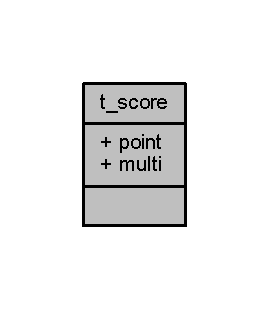
\includegraphics[width=129pt]{d6/db1/structt__score__coll__graph}
\end{center}
\end{figure}
\subsection*{Champs de données}
\begin{DoxyCompactItemize}
\item 
int \hyperlink{structt__score_a2dee8b7fcecc7c2d190e9304b43ea886}{point}
\item 
int \hyperlink{structt__score_a75308cd0de4d855ff6cb9baec37dddde}{multi}
\end{DoxyCompactItemize}


\subsection{Description détaillée}
défini le score du mot que l\textquotesingle{}on est en train de chercher. 

Définition à la ligne 47 du fichier ruzzle.\+h.



\subsection{Documentation des champs}
\hypertarget{structt__score_a75308cd0de4d855ff6cb9baec37dddde}{}\index{t\+\_\+score@{t\+\_\+score}!multi@{multi}}
\index{multi@{multi}!t\+\_\+score@{t\+\_\+score}}
\subsubsection[{multi}]{\setlength{\rightskip}{0pt plus 5cm}int multi}\label{structt__score_a75308cd0de4d855ff6cb9baec37dddde}


Définition à la ligne 50 du fichier ruzzle.\+h.

\hypertarget{structt__score_a2dee8b7fcecc7c2d190e9304b43ea886}{}\index{t\+\_\+score@{t\+\_\+score}!point@{point}}
\index{point@{point}!t\+\_\+score@{t\+\_\+score}}
\subsubsection[{point}]{\setlength{\rightskip}{0pt plus 5cm}int point}\label{structt__score_a2dee8b7fcecc7c2d190e9304b43ea886}


Définition à la ligne 49 du fichier ruzzle.\+h.



La documentation de cette structure a été générée à partir du fichier suivant \+:\begin{DoxyCompactItemize}
\item 
\hyperlink{ruzzle_8h}{ruzzle.\+h}\end{DoxyCompactItemize}

\chapter{Documentation des fichiers}
\hypertarget{liste_8c}{}\section{Référence du fichier liste.\+c}
\label{liste_8c}\index{liste.\+c@{liste.\+c}}


Programme de gestion d\textquotesingle{}une liste.  


{\ttfamily \#include $<$stdlib.\+h$>$}\\*
{\ttfamily \#include $<$stdio.\+h$>$}\\*
{\ttfamily \#include $<$stdbool.\+h$>$}\\*
{\ttfamily \#include $<$string.\+h$>$}\\*
Graphe des dépendances par inclusion de liste.\+c\+:
\nopagebreak
\begin{figure}[H]
\begin{center}
\leavevmode
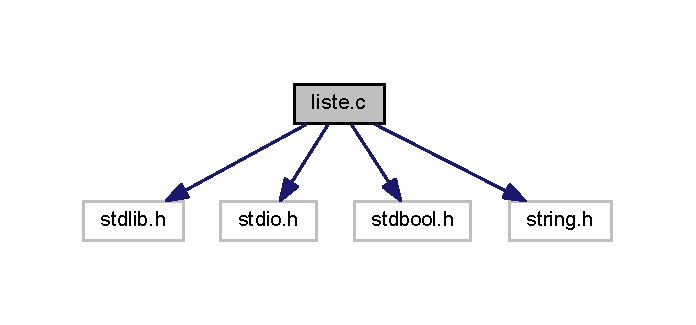
\includegraphics[width=334pt]{d2/d3f/liste_8c__incl}
\end{center}
\end{figure}
\subsection*{Structures de données}
\begin{DoxyCompactItemize}
\item 
struct \hyperlink{structelement}{element}
\begin{DoxyCompactList}\small\item\em Structure de donnée formant un élément de la liste. \end{DoxyCompactList}\end{DoxyCompactItemize}
\subsection*{Définitions de type}
\begin{DoxyCompactItemize}
\item 
typedef struct \hyperlink{structelement}{element} \hyperlink{liste_8c_aaa9f09bf55fb32a9090e2dc051b75a6a}{t\+\_\+element}
\begin{DoxyCompactList}\small\item\em Structure de donnée formant un élément de la liste. \end{DoxyCompactList}\end{DoxyCompactItemize}
\subsection*{Fonctions}
\begin{DoxyCompactItemize}
\item 
void \hyperlink{liste_8c_a4fe6a1e67a4e3ed6e67a91704873d7c2}{init\+\_\+liste} (void)
\begin{DoxyCompactList}\small\item\em Initialise la liste à vide. \end{DoxyCompactList}\item 
bool \hyperlink{liste_8c_a7c1f2e07788b9e73ec80a044c36d5231}{liste\+\_\+vide} (void)
\begin{DoxyCompactList}\small\item\em Fonction permettant de savoir si la liste contient au moins un element. \end{DoxyCompactList}\item 
bool \hyperlink{liste_8c_ab280062aa7789f70bc0436edd0c674cd}{hors\+\_\+liste} (void)
\begin{DoxyCompactList}\small\item\em Verifie si on se trouve encore dans la liste. \end{DoxyCompactList}\item 
void \hyperlink{liste_8c_a68274781c5c541e03951b5e3f408e1d2}{en\+\_\+tete} (void)
\begin{DoxyCompactList}\small\item\em Positionne en tete de la liste. \end{DoxyCompactList}\item 
void \hyperlink{liste_8c_aaacc4277d423e99a9c929cdadb00a65c}{en\+\_\+queue} (void)
\begin{DoxyCompactList}\small\item\em Positionne en queue de la liste. \end{DoxyCompactList}\item 
void \hyperlink{liste_8c_a5cd9c9ae9a2d39e81678f35d50540d36}{suivant} (void)
\begin{DoxyCompactList}\small\item\em Positionne sur l\textquotesingle{}element suivant. \end{DoxyCompactList}\item 
void \hyperlink{liste_8c_afa1ade166b772261d348f25527fa3f29}{valeur\+\_\+elt} (char mot\mbox{[}20\mbox{]}, int $\ast$score)
\begin{DoxyCompactList}\small\item\em Renvoi les valeurs comprises dans l\textquotesingle{}element courant. \end{DoxyCompactList}\item 
void \hyperlink{liste_8c_ae5922bfd958a4a1bbfee1cb8c2756684}{ajout\+\_\+droit} (char $\ast$in\+Word, int score)
\begin{DoxyCompactList}\small\item\em Ajoute un nouvel élément a droite de l\textquotesingle{}elt courant. \end{DoxyCompactList}\item 
void \hyperlink{liste_8c_a87ff26aaf018f7d1cc2a926aea1d488a}{ajout\+\_\+gauche} (char $\ast$in\+Word, int score)
\begin{DoxyCompactList}\small\item\em Ajoute un nouvel élément a gauche de l\textquotesingle{}elt courant. \end{DoxyCompactList}\end{DoxyCompactItemize}
\subsection*{Variables}
\begin{DoxyCompactItemize}
\item 
\hyperlink{liste_8c_aaa9f09bf55fb32a9090e2dc051b75a6a}{t\+\_\+element} $\ast$ \hyperlink{liste_8c_a0c3bc65023967a457d3f8427649fb965}{drapeau}
\item 
\hyperlink{liste_8c_aaa9f09bf55fb32a9090e2dc051b75a6a}{t\+\_\+element} $\ast$ \hyperlink{liste_8c_a33528e825c99db5ca765f2d8c9b1340e}{ec}
\end{DoxyCompactItemize}


\subsection{Description détaillée}
Programme de gestion d\textquotesingle{}une liste. 

\begin{DoxyAuthor}{Auteur}
Ewen C. Bastien B. 
\end{DoxyAuthor}
\begin{DoxyVersion}{Version}
1.\+0 
\end{DoxyVersion}
\begin{DoxyDate}{Date}
22/11/2015
\end{DoxyDate}
Gestion d\textquotesingle{}une liste doublement chainée contenant une chaine de caractère et un entier 

\subsection{Documentation des définitions de type}
\hypertarget{liste_8c_aaa9f09bf55fb32a9090e2dc051b75a6a}{}\index{liste.\+c@{liste.\+c}!t\+\_\+element@{t\+\_\+element}}
\index{t\+\_\+element@{t\+\_\+element}!liste.\+c@{liste.\+c}}
\subsubsection[{t\+\_\+element}]{\setlength{\rightskip}{0pt plus 5cm}typedef struct {\bf element} {\bf t\+\_\+element}}\label{liste_8c_aaa9f09bf55fb32a9090e2dc051b75a6a}


Structure de donnée formant un élément de la liste. 



\subsection{Documentation des fonctions}
\hypertarget{liste_8c_ae5922bfd958a4a1bbfee1cb8c2756684}{}\index{liste.\+c@{liste.\+c}!ajout\+\_\+droit@{ajout\+\_\+droit}}
\index{ajout\+\_\+droit@{ajout\+\_\+droit}!liste.\+c@{liste.\+c}}
\subsubsection[{ajout\+\_\+droit(char $\ast$in\+Word, int score)}]{\setlength{\rightskip}{0pt plus 5cm}void ajout\+\_\+droit (
\begin{DoxyParamCaption}
\item[{char $\ast$}]{in\+Word, }
\item[{int}]{score}
\end{DoxyParamCaption}
)}\label{liste_8c_ae5922bfd958a4a1bbfee1cb8c2756684}


Ajoute un nouvel élément a droite de l\textquotesingle{}elt courant. 


\begin{DoxyParams}{Paramètres}
{\em in\+Word} & \+: Mot à ajouter \\
\hline
{\em score} & \+: Score à ajouter \\
\hline
\end{DoxyParams}


Définition à la ligne 129 du fichier liste.\+c.



Voici le graphe d\textquotesingle{}appel pour cette fonction \+:
\nopagebreak
\begin{figure}[H]
\begin{center}
\leavevmode
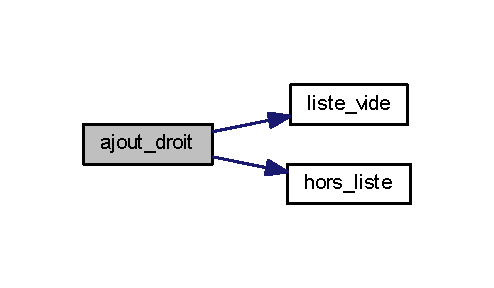
\includegraphics[width=237pt]{d3/dc8/liste_8c_ae5922bfd958a4a1bbfee1cb8c2756684_cgraph}
\end{center}
\end{figure}


\hypertarget{liste_8c_a87ff26aaf018f7d1cc2a926aea1d488a}{}\index{liste.\+c@{liste.\+c}!ajout\+\_\+gauche@{ajout\+\_\+gauche}}
\index{ajout\+\_\+gauche@{ajout\+\_\+gauche}!liste.\+c@{liste.\+c}}
\subsubsection[{ajout\+\_\+gauche(char $\ast$in\+Word, int score)}]{\setlength{\rightskip}{0pt plus 5cm}void ajout\+\_\+gauche (
\begin{DoxyParamCaption}
\item[{char $\ast$}]{in\+Word, }
\item[{int}]{score}
\end{DoxyParamCaption}
)}\label{liste_8c_a87ff26aaf018f7d1cc2a926aea1d488a}


Ajoute un nouvel élément a gauche de l\textquotesingle{}elt courant. 


\begin{DoxyParams}{Paramètres}
{\em in\+Word} & \+: Mot à ajouter \\
\hline
{\em score} & \+: Score à ajouter \\
\hline
\end{DoxyParams}


Définition à la ligne 153 du fichier liste.\+c.



Voici le graphe d\textquotesingle{}appel pour cette fonction \+:
\nopagebreak
\begin{figure}[H]
\begin{center}
\leavevmode
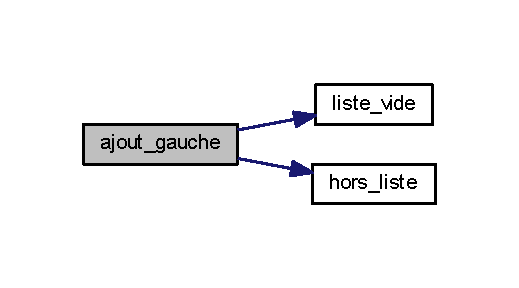
\includegraphics[width=249pt]{d3/dc8/liste_8c_a87ff26aaf018f7d1cc2a926aea1d488a_cgraph}
\end{center}
\end{figure}


\hypertarget{liste_8c_aaacc4277d423e99a9c929cdadb00a65c}{}\index{liste.\+c@{liste.\+c}!en\+\_\+queue@{en\+\_\+queue}}
\index{en\+\_\+queue@{en\+\_\+queue}!liste.\+c@{liste.\+c}}
\subsubsection[{en\+\_\+queue(void)}]{\setlength{\rightskip}{0pt plus 5cm}void en\+\_\+queue (
\begin{DoxyParamCaption}
\item[{void}]{}
\end{DoxyParamCaption}
)}\label{liste_8c_aaacc4277d423e99a9c929cdadb00a65c}


Positionne en queue de la liste. 



Définition à la ligne 89 du fichier liste.\+c.



Voici le graphe d\textquotesingle{}appel pour cette fonction \+:
\nopagebreak
\begin{figure}[H]
\begin{center}
\leavevmode
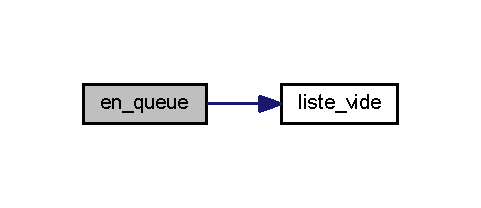
\includegraphics[width=231pt]{d3/dc8/liste_8c_aaacc4277d423e99a9c929cdadb00a65c_cgraph}
\end{center}
\end{figure}


\hypertarget{liste_8c_a68274781c5c541e03951b5e3f408e1d2}{}\index{liste.\+c@{liste.\+c}!en\+\_\+tete@{en\+\_\+tete}}
\index{en\+\_\+tete@{en\+\_\+tete}!liste.\+c@{liste.\+c}}
\subsubsection[{en\+\_\+tete(void)}]{\setlength{\rightskip}{0pt plus 5cm}void en\+\_\+tete (
\begin{DoxyParamCaption}
\item[{void}]{}
\end{DoxyParamCaption}
)}\label{liste_8c_a68274781c5c541e03951b5e3f408e1d2}


Positionne en tete de la liste. 



Définition à la ligne 78 du fichier liste.\+c.



Voici le graphe d\textquotesingle{}appel pour cette fonction \+:
\nopagebreak
\begin{figure}[H]
\begin{center}
\leavevmode
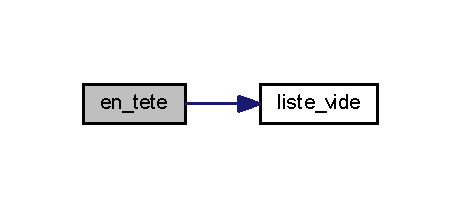
\includegraphics[width=221pt]{d3/dc8/liste_8c_a68274781c5c541e03951b5e3f408e1d2_cgraph}
\end{center}
\end{figure}


\hypertarget{liste_8c_ab280062aa7789f70bc0436edd0c674cd}{}\index{liste.\+c@{liste.\+c}!hors\+\_\+liste@{hors\+\_\+liste}}
\index{hors\+\_\+liste@{hors\+\_\+liste}!liste.\+c@{liste.\+c}}
\subsubsection[{hors\+\_\+liste(void)}]{\setlength{\rightskip}{0pt plus 5cm}bool hors\+\_\+liste (
\begin{DoxyParamCaption}
\item[{void}]{}
\end{DoxyParamCaption}
)}\label{liste_8c_ab280062aa7789f70bc0436edd0c674cd}


Verifie si on se trouve encore dans la liste. 

\begin{DoxyReturn}{Renvoie}
Renvoi un booleen à vrai si l\textquotesingle{}element courant est hors de la liste, faux sinon. 
\end{DoxyReturn}


Définition à la ligne 68 du fichier liste.\+c.

\hypertarget{liste_8c_a4fe6a1e67a4e3ed6e67a91704873d7c2}{}\index{liste.\+c@{liste.\+c}!init\+\_\+liste@{init\+\_\+liste}}
\index{init\+\_\+liste@{init\+\_\+liste}!liste.\+c@{liste.\+c}}
\subsubsection[{init\+\_\+liste(void)}]{\setlength{\rightskip}{0pt plus 5cm}void init\+\_\+liste (
\begin{DoxyParamCaption}
\item[{void}]{}
\end{DoxyParamCaption}
)}\label{liste_8c_a4fe6a1e67a4e3ed6e67a91704873d7c2}


Initialise la liste à vide. 



Définition à la ligne 41 du fichier liste.\+c.

\hypertarget{liste_8c_a7c1f2e07788b9e73ec80a044c36d5231}{}\index{liste.\+c@{liste.\+c}!liste\+\_\+vide@{liste\+\_\+vide}}
\index{liste\+\_\+vide@{liste\+\_\+vide}!liste.\+c@{liste.\+c}}
\subsubsection[{liste\+\_\+vide(void)}]{\setlength{\rightskip}{0pt plus 5cm}bool liste\+\_\+vide (
\begin{DoxyParamCaption}
\item[{void}]{}
\end{DoxyParamCaption}
)}\label{liste_8c_a7c1f2e07788b9e73ec80a044c36d5231}


Fonction permettant de savoir si la liste contient au moins un element. 

\begin{DoxyReturn}{Renvoie}
Renvoi un booléen à vrai si la liste est vide, faux sinon. 
\end{DoxyReturn}


Définition à la ligne 56 du fichier liste.\+c.

\hypertarget{liste_8c_a5cd9c9ae9a2d39e81678f35d50540d36}{}\index{liste.\+c@{liste.\+c}!suivant@{suivant}}
\index{suivant@{suivant}!liste.\+c@{liste.\+c}}
\subsubsection[{suivant(void)}]{\setlength{\rightskip}{0pt plus 5cm}void suivant (
\begin{DoxyParamCaption}
\item[{void}]{}
\end{DoxyParamCaption}
)}\label{liste_8c_a5cd9c9ae9a2d39e81678f35d50540d36}


Positionne sur l\textquotesingle{}element suivant. 



Définition à la ligne 100 du fichier liste.\+c.



Voici le graphe d\textquotesingle{}appel pour cette fonction \+:
\nopagebreak
\begin{figure}[H]
\begin{center}
\leavevmode
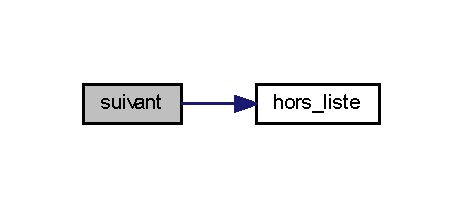
\includegraphics[width=222pt]{d3/dc8/liste_8c_a5cd9c9ae9a2d39e81678f35d50540d36_cgraph}
\end{center}
\end{figure}


\hypertarget{liste_8c_afa1ade166b772261d348f25527fa3f29}{}\index{liste.\+c@{liste.\+c}!valeur\+\_\+elt@{valeur\+\_\+elt}}
\index{valeur\+\_\+elt@{valeur\+\_\+elt}!liste.\+c@{liste.\+c}}
\subsubsection[{valeur\+\_\+elt(char mot[20], int $\ast$score)}]{\setlength{\rightskip}{0pt plus 5cm}void valeur\+\_\+elt (
\begin{DoxyParamCaption}
\item[{char}]{mot\mbox{[}20\mbox{]}, }
\item[{int $\ast$}]{score}
\end{DoxyParamCaption}
)}\label{liste_8c_afa1ade166b772261d348f25527fa3f29}


Renvoi les valeurs comprises dans l\textquotesingle{}element courant. 


\begin{DoxyParams}{Paramètres}
{\em mot} & \+: Le mot enregistré dans la liste \\
\hline
{\em score} & \+: Le score enregistré dans la liste \\
\hline
\end{DoxyParams}


Définition à la ligne 114 du fichier liste.\+c.



Voici le graphe d\textquotesingle{}appel pour cette fonction \+:
\nopagebreak
\begin{figure}[H]
\begin{center}
\leavevmode
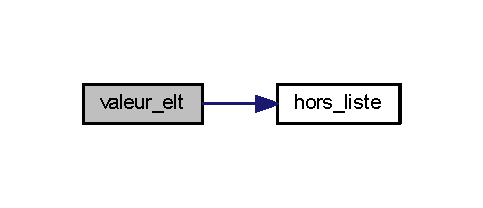
\includegraphics[width=232pt]{d3/dc8/liste_8c_afa1ade166b772261d348f25527fa3f29_cgraph}
\end{center}
\end{figure}




\subsection{Documentation des variables}
\hypertarget{liste_8c_a0c3bc65023967a457d3f8427649fb965}{}\index{liste.\+c@{liste.\+c}!drapeau@{drapeau}}
\index{drapeau@{drapeau}!liste.\+c@{liste.\+c}}
\subsubsection[{drapeau}]{\setlength{\rightskip}{0pt plus 5cm}{\bf t\+\_\+element}$\ast$ drapeau}\label{liste_8c_a0c3bc65023967a457d3f8427649fb965}
Pointeur sur l\textquotesingle{}élément initial de la liste. 

Définition à la ligne 33 du fichier liste.\+c.

\hypertarget{liste_8c_a33528e825c99db5ca765f2d8c9b1340e}{}\index{liste.\+c@{liste.\+c}!ec@{ec}}
\index{ec@{ec}!liste.\+c@{liste.\+c}}
\subsubsection[{ec}]{\setlength{\rightskip}{0pt plus 5cm}{\bf t\+\_\+element}$\ast$ ec}\label{liste_8c_a33528e825c99db5ca765f2d8c9b1340e}
Pointeur sur l\textquotesingle{}élément courant de la liste. 

Définition à la ligne 34 du fichier liste.\+c.


\hypertarget{liste_8h}{}\section{Référence du fichier liste.\+h}
\label{liste_8h}\index{liste.\+h@{liste.\+h}}
Ce graphe montre quels fichiers incluent directement ou indirectement ce fichier \+:
\nopagebreak
\begin{figure}[H]
\begin{center}
\leavevmode
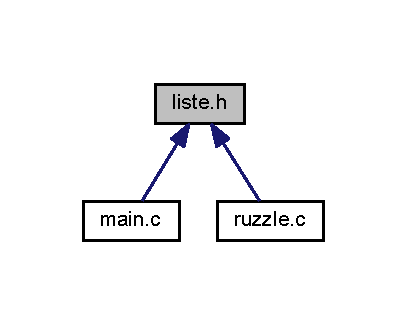
\includegraphics[width=196pt]{dd/d4e/liste_8h__dep__incl}
\end{center}
\end{figure}
\subsection*{Fonctions}
\begin{DoxyCompactItemize}
\item 
void \hyperlink{liste_8h_a4fe6a1e67a4e3ed6e67a91704873d7c2}{init\+\_\+liste} (void)
\begin{DoxyCompactList}\small\item\em Initialise la liste à vide. \end{DoxyCompactList}\item 
bool \hyperlink{liste_8h_a7c1f2e07788b9e73ec80a044c36d5231}{liste\+\_\+vide} (void)
\begin{DoxyCompactList}\small\item\em Fonction permettant de savoir si la liste contient au moins un element. \end{DoxyCompactList}\item 
bool \hyperlink{liste_8h_ab280062aa7789f70bc0436edd0c674cd}{hors\+\_\+liste} (void)
\begin{DoxyCompactList}\small\item\em Verifie si on se trouve encore dans la liste. \end{DoxyCompactList}\item 
void \hyperlink{liste_8h_a68274781c5c541e03951b5e3f408e1d2}{en\+\_\+tete} (void)
\begin{DoxyCompactList}\small\item\em Positionne en tete de la liste. \end{DoxyCompactList}\item 
void \hyperlink{liste_8h_aaacc4277d423e99a9c929cdadb00a65c}{en\+\_\+queue} (void)
\begin{DoxyCompactList}\small\item\em Positionne en queue de la liste. \end{DoxyCompactList}\item 
void \hyperlink{liste_8h_a5cd9c9ae9a2d39e81678f35d50540d36}{suivant} (void)
\begin{DoxyCompactList}\small\item\em Positionne sur l\textquotesingle{}element suivant. \end{DoxyCompactList}\item 
void \hyperlink{liste_8h_af9745ed4b29394b89f32a7598ce80365}{valeur\+\_\+elt} (char\mbox{[}$\,$\mbox{]}, int $\ast$)
\item 
void \hyperlink{liste_8h_a483769044edc043258a1560fdc351e5a}{ajout\+\_\+droit} (char $\ast$, int)
\begin{DoxyCompactList}\small\item\em Ajoute un nouvel élément a droite de l\textquotesingle{}elt courant. \end{DoxyCompactList}\item 
void \hyperlink{liste_8h_ad2e1a24934fb93e4fcb8e58f351b5ffb}{ajout\+\_\+gauche} (char $\ast$, int)
\begin{DoxyCompactList}\small\item\em Ajoute un nouvel élément a gauche de l\textquotesingle{}elt courant. \end{DoxyCompactList}\end{DoxyCompactItemize}


\subsection{Documentation des fonctions}
\hypertarget{liste_8h_a483769044edc043258a1560fdc351e5a}{}\index{liste.\+h@{liste.\+h}!ajout\+\_\+droit@{ajout\+\_\+droit}}
\index{ajout\+\_\+droit@{ajout\+\_\+droit}!liste.\+h@{liste.\+h}}
\subsubsection[{ajout\+\_\+droit(char $\ast$, int)}]{\setlength{\rightskip}{0pt plus 5cm}void ajout\+\_\+droit (
\begin{DoxyParamCaption}
\item[{char $\ast$}]{in\+Word, }
\item[{int}]{score}
\end{DoxyParamCaption}
)}\label{liste_8h_a483769044edc043258a1560fdc351e5a}


Ajoute un nouvel élément a droite de l\textquotesingle{}elt courant. 


\begin{DoxyParams}{Paramètres}
{\em in\+Word} & \+: Mot à ajouter \\
\hline
{\em score} & \+: Score à ajouter \\
\hline
\end{DoxyParams}


Définition à la ligne 129 du fichier liste.\+c.



Voici le graphe d\textquotesingle{}appel pour cette fonction \+:
\nopagebreak
\begin{figure}[H]
\begin{center}
\leavevmode
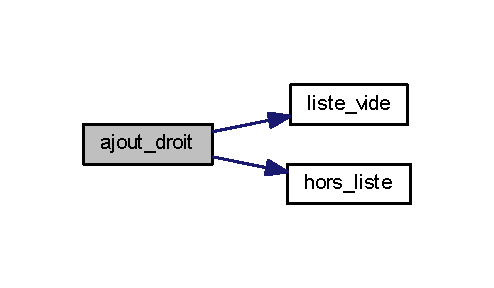
\includegraphics[width=237pt]{d4/d5b/liste_8h_a483769044edc043258a1560fdc351e5a_cgraph}
\end{center}
\end{figure}


\hypertarget{liste_8h_ad2e1a24934fb93e4fcb8e58f351b5ffb}{}\index{liste.\+h@{liste.\+h}!ajout\+\_\+gauche@{ajout\+\_\+gauche}}
\index{ajout\+\_\+gauche@{ajout\+\_\+gauche}!liste.\+h@{liste.\+h}}
\subsubsection[{ajout\+\_\+gauche(char $\ast$, int)}]{\setlength{\rightskip}{0pt plus 5cm}void ajout\+\_\+gauche (
\begin{DoxyParamCaption}
\item[{char $\ast$}]{in\+Word, }
\item[{int}]{score}
\end{DoxyParamCaption}
)}\label{liste_8h_ad2e1a24934fb93e4fcb8e58f351b5ffb}


Ajoute un nouvel élément a gauche de l\textquotesingle{}elt courant. 


\begin{DoxyParams}{Paramètres}
{\em in\+Word} & \+: Mot à ajouter \\
\hline
{\em score} & \+: Score à ajouter \\
\hline
\end{DoxyParams}


Définition à la ligne 153 du fichier liste.\+c.



Voici le graphe d\textquotesingle{}appel pour cette fonction \+:
\nopagebreak
\begin{figure}[H]
\begin{center}
\leavevmode
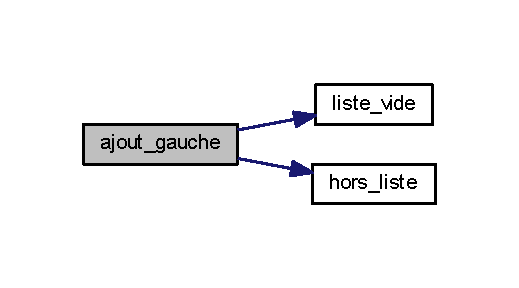
\includegraphics[width=249pt]{d4/d5b/liste_8h_ad2e1a24934fb93e4fcb8e58f351b5ffb_cgraph}
\end{center}
\end{figure}


\hypertarget{liste_8h_aaacc4277d423e99a9c929cdadb00a65c}{}\index{liste.\+h@{liste.\+h}!en\+\_\+queue@{en\+\_\+queue}}
\index{en\+\_\+queue@{en\+\_\+queue}!liste.\+h@{liste.\+h}}
\subsubsection[{en\+\_\+queue(void)}]{\setlength{\rightskip}{0pt plus 5cm}void en\+\_\+queue (
\begin{DoxyParamCaption}
\item[{void}]{}
\end{DoxyParamCaption}
)}\label{liste_8h_aaacc4277d423e99a9c929cdadb00a65c}


Positionne en queue de la liste. 



Définition à la ligne 89 du fichier liste.\+c.



Voici le graphe d\textquotesingle{}appel pour cette fonction \+:
\nopagebreak
\begin{figure}[H]
\begin{center}
\leavevmode
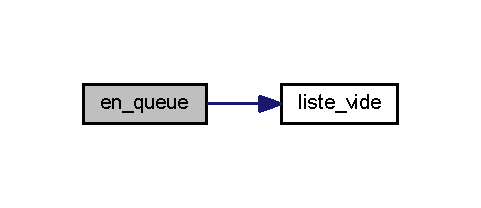
\includegraphics[width=231pt]{d4/d5b/liste_8h_aaacc4277d423e99a9c929cdadb00a65c_cgraph}
\end{center}
\end{figure}


\hypertarget{liste_8h_a68274781c5c541e03951b5e3f408e1d2}{}\index{liste.\+h@{liste.\+h}!en\+\_\+tete@{en\+\_\+tete}}
\index{en\+\_\+tete@{en\+\_\+tete}!liste.\+h@{liste.\+h}}
\subsubsection[{en\+\_\+tete(void)}]{\setlength{\rightskip}{0pt plus 5cm}void en\+\_\+tete (
\begin{DoxyParamCaption}
\item[{void}]{}
\end{DoxyParamCaption}
)}\label{liste_8h_a68274781c5c541e03951b5e3f408e1d2}


Positionne en tete de la liste. 



Définition à la ligne 78 du fichier liste.\+c.



Voici le graphe d\textquotesingle{}appel pour cette fonction \+:
\nopagebreak
\begin{figure}[H]
\begin{center}
\leavevmode
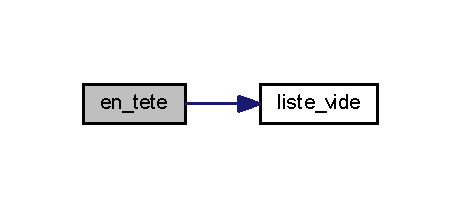
\includegraphics[width=221pt]{d4/d5b/liste_8h_a68274781c5c541e03951b5e3f408e1d2_cgraph}
\end{center}
\end{figure}


\hypertarget{liste_8h_ab280062aa7789f70bc0436edd0c674cd}{}\index{liste.\+h@{liste.\+h}!hors\+\_\+liste@{hors\+\_\+liste}}
\index{hors\+\_\+liste@{hors\+\_\+liste}!liste.\+h@{liste.\+h}}
\subsubsection[{hors\+\_\+liste(void)}]{\setlength{\rightskip}{0pt plus 5cm}bool hors\+\_\+liste (
\begin{DoxyParamCaption}
\item[{void}]{}
\end{DoxyParamCaption}
)}\label{liste_8h_ab280062aa7789f70bc0436edd0c674cd}


Verifie si on se trouve encore dans la liste. 

\begin{DoxyReturn}{Renvoie}
Renvoi un booleen à vrai si l\textquotesingle{}element courant est hors de la liste, faux sinon. 
\end{DoxyReturn}


Définition à la ligne 68 du fichier liste.\+c.

\hypertarget{liste_8h_a4fe6a1e67a4e3ed6e67a91704873d7c2}{}\index{liste.\+h@{liste.\+h}!init\+\_\+liste@{init\+\_\+liste}}
\index{init\+\_\+liste@{init\+\_\+liste}!liste.\+h@{liste.\+h}}
\subsubsection[{init\+\_\+liste(void)}]{\setlength{\rightskip}{0pt plus 5cm}void init\+\_\+liste (
\begin{DoxyParamCaption}
\item[{void}]{}
\end{DoxyParamCaption}
)}\label{liste_8h_a4fe6a1e67a4e3ed6e67a91704873d7c2}


Initialise la liste à vide. 



Définition à la ligne 41 du fichier liste.\+c.

\hypertarget{liste_8h_a7c1f2e07788b9e73ec80a044c36d5231}{}\index{liste.\+h@{liste.\+h}!liste\+\_\+vide@{liste\+\_\+vide}}
\index{liste\+\_\+vide@{liste\+\_\+vide}!liste.\+h@{liste.\+h}}
\subsubsection[{liste\+\_\+vide(void)}]{\setlength{\rightskip}{0pt plus 5cm}bool liste\+\_\+vide (
\begin{DoxyParamCaption}
\item[{void}]{}
\end{DoxyParamCaption}
)}\label{liste_8h_a7c1f2e07788b9e73ec80a044c36d5231}


Fonction permettant de savoir si la liste contient au moins un element. 

\begin{DoxyReturn}{Renvoie}
Renvoi un booléen à vrai si la liste est vide, faux sinon. 
\end{DoxyReturn}


Définition à la ligne 56 du fichier liste.\+c.

\hypertarget{liste_8h_a5cd9c9ae9a2d39e81678f35d50540d36}{}\index{liste.\+h@{liste.\+h}!suivant@{suivant}}
\index{suivant@{suivant}!liste.\+h@{liste.\+h}}
\subsubsection[{suivant(void)}]{\setlength{\rightskip}{0pt plus 5cm}void suivant (
\begin{DoxyParamCaption}
\item[{void}]{}
\end{DoxyParamCaption}
)}\label{liste_8h_a5cd9c9ae9a2d39e81678f35d50540d36}


Positionne sur l\textquotesingle{}element suivant. 



Définition à la ligne 100 du fichier liste.\+c.



Voici le graphe d\textquotesingle{}appel pour cette fonction \+:
\nopagebreak
\begin{figure}[H]
\begin{center}
\leavevmode
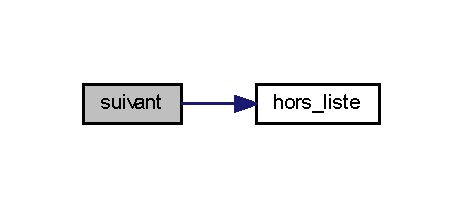
\includegraphics[width=222pt]{d4/d5b/liste_8h_a5cd9c9ae9a2d39e81678f35d50540d36_cgraph}
\end{center}
\end{figure}


\hypertarget{liste_8h_af9745ed4b29394b89f32a7598ce80365}{}\index{liste.\+h@{liste.\+h}!valeur\+\_\+elt@{valeur\+\_\+elt}}
\index{valeur\+\_\+elt@{valeur\+\_\+elt}!liste.\+h@{liste.\+h}}
\subsubsection[{valeur\+\_\+elt(char[], int $\ast$)}]{\setlength{\rightskip}{0pt plus 5cm}void valeur\+\_\+elt (
\begin{DoxyParamCaption}
\item[{char}]{\mbox{[}$\,$\mbox{]}, }
\item[{int $\ast$}]{}
\end{DoxyParamCaption}
)}\label{liste_8h_af9745ed4b29394b89f32a7598ce80365}

\hypertarget{main_8c}{}\section{Référence du fichier main.\+c}
\label{main_8c}\index{main.\+c@{main.\+c}}


Programme principal.  


{\ttfamily \#include $<$stdio.\+h$>$}\\*
{\ttfamily \#include $<$stdlib.\+h$>$}\\*
{\ttfamily \#include $<$string.\+h$>$}\\*
{\ttfamily \#include $<$stdbool.\+h$>$}\\*
{\ttfamily \#include $<$ctype.\+h$>$}\\*
{\ttfamily \#include \char`\"{}liste.\+h\char`\"{}}\\*
{\ttfamily \#include \char`\"{}ruzzle.\+h\char`\"{}}\\*
Graphe des dépendances par inclusion de main.\+c\+:
\nopagebreak
\begin{figure}[H]
\begin{center}
\leavevmode
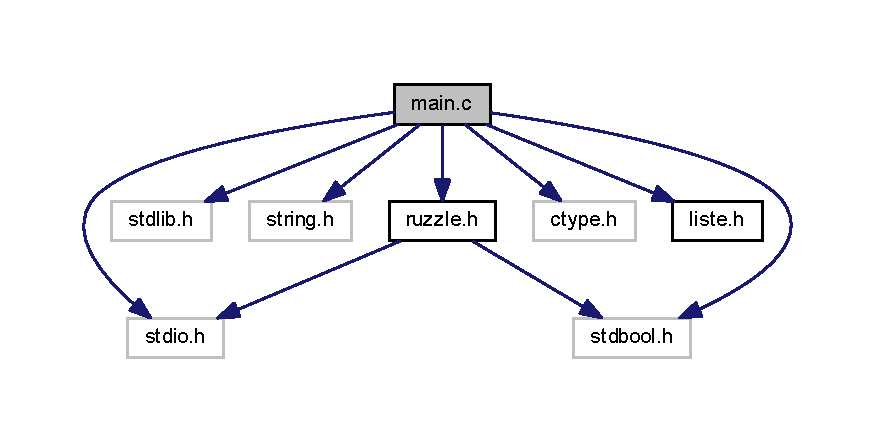
\includegraphics[width=350pt]{d4/d10/main_8c__incl}
\end{center}
\end{figure}
\subsection*{Macros}
\begin{DoxyCompactItemize}
\item 
\#define \hyperlink{main_8c_a0240ac851181b84ac374872dc5434ee4}{N}~4
\end{DoxyCompactItemize}
\subsection*{Fonctions}
\begin{DoxyCompactItemize}
\item 
int \hyperlink{main_8c_a0ddf1224851353fc92bfbff6f499fa97}{main} (int argc, char $\ast$argv\mbox{[}$\,$\mbox{]})
\end{DoxyCompactItemize}


\subsection{Description détaillée}
Programme principal. 

\begin{DoxyAuthor}{Auteur}
Ewen C. Bastien B. 
\end{DoxyAuthor}
\begin{DoxyVersion}{Version}
1.\+0 
\end{DoxyVersion}
\begin{DoxyDate}{Date}
22/11/2015
\end{DoxyDate}
Programme initialisant les structure et fichiers et appelant les fonctions filles. 

\subsection{Documentation des macros}
\hypertarget{main_8c_a0240ac851181b84ac374872dc5434ee4}{}\index{main.\+c@{main.\+c}!N@{N}}
\index{N@{N}!main.\+c@{main.\+c}}
\subsubsection[{N}]{\setlength{\rightskip}{0pt plus 5cm}\#define N~4}\label{main_8c_a0240ac851181b84ac374872dc5434ee4}


Définition à la ligne 21 du fichier main.\+c.



\subsection{Documentation des fonctions}
\hypertarget{main_8c_a0ddf1224851353fc92bfbff6f499fa97}{}\index{main.\+c@{main.\+c}!main@{main}}
\index{main@{main}!main.\+c@{main.\+c}}
\subsubsection[{main(int argc, char $\ast$argv[])}]{\setlength{\rightskip}{0pt plus 5cm}int main (
\begin{DoxyParamCaption}
\item[{int}]{argc, }
\item[{char $\ast$}]{argv\mbox{[}$\,$\mbox{]}}
\end{DoxyParamCaption}
)}\label{main_8c_a0ddf1224851353fc92bfbff6f499fa97}


Définition à la ligne 23 du fichier main.\+c.



Voici le graphe d\textquotesingle{}appel pour cette fonction \+:
\nopagebreak
\begin{figure}[H]
\begin{center}
\leavevmode
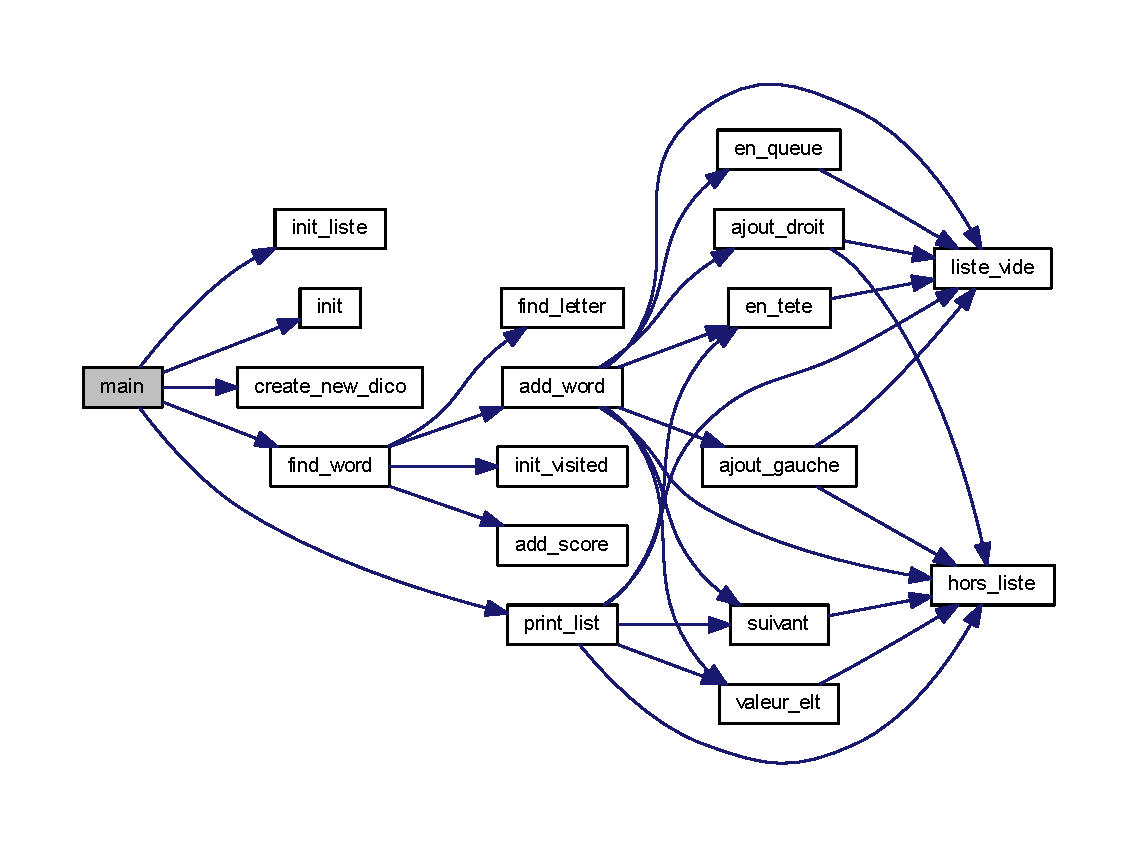
\includegraphics[width=350pt]{d0/d29/main_8c_a0ddf1224851353fc92bfbff6f499fa97_cgraph}
\end{center}
\end{figure}



\hypertarget{_r_e_a_d_m_e_8md}{}\section{Référence du fichier R\+E\+A\+D\+M\+E.\+md}
\label{_r_e_a_d_m_e_8md}\index{R\+E\+A\+D\+M\+E.\+md@{R\+E\+A\+D\+M\+E.\+md}}

\hypertarget{ruzzle_8c}{}\section{Référence du fichier ruzzle.\+c}
\label{ruzzle_8c}\index{ruzzle.\+c@{ruzzle.\+c}}


Fonctions du ruzzle solver.  


{\ttfamily \#include $<$string.\+h$>$}\\*
{\ttfamily \#include $<$ctype.\+h$>$}\\*
{\ttfamily \#include \char`\"{}ruzzle.\+h\char`\"{}}\\*
{\ttfamily \#include \char`\"{}liste.\+h\char`\"{}}\\*
Graphe des dépendances par inclusion de ruzzle.\+c\+:
\nopagebreak
\begin{figure}[H]
\begin{center}
\leavevmode
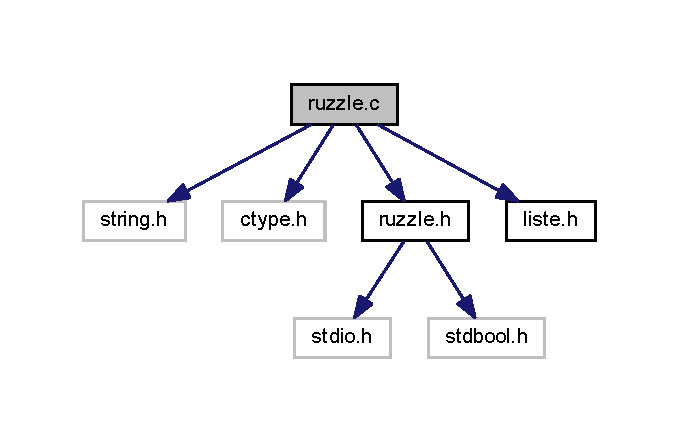
\includegraphics[width=326pt]{df/d55/ruzzle_8c__incl}
\end{center}
\end{figure}
\subsection*{Fonctions}
\begin{DoxyCompactItemize}
\item 
int \hyperlink{ruzzle_8c_a17b31853d3aa79a67d0c25a3ae68a89a}{init} (char entree\mbox{[}$\,$\mbox{]}, \hyperlink{structcell}{cell} sortie\mbox{[}\hyperlink{ruzzle_8h_a0240ac851181b84ac374872dc5434ee4}{N}\mbox{]}\mbox{[}\hyperlink{ruzzle_8h_a0240ac851181b84ac374872dc5434ee4}{N}\mbox{]}, F\+I\+L\+E $\ast$dico, F\+I\+L\+E $\ast$output)
\begin{DoxyCompactList}\small\item\em Fonction d\textquotesingle{}initialisation globale. \end{DoxyCompactList}\item 
int \hyperlink{ruzzle_8c_a718478def452ab5bca4b1a3bc8393c57}{create\+\_\+new\+\_\+dico} (\hyperlink{structcell}{cell} ruzzle\mbox{[}\hyperlink{ruzzle_8h_a0240ac851181b84ac374872dc5434ee4}{N}\mbox{]}\mbox{[}\hyperlink{ruzzle_8h_a0240ac851181b84ac374872dc5434ee4}{N}\mbox{]}, F\+I\+L\+E $\ast$dico)
\begin{DoxyCompactList}\small\item\em Crée un dictionaire élagué \end{DoxyCompactList}\item 
bool \hyperlink{ruzzle_8c_ad285e4b1ee303ca9809b0aeb31d62685}{find\+\_\+letter} (char c, \hyperlink{structcoord}{coord} $\ast$pos, \hyperlink{structcell}{cell} ruzzle\mbox{[}\hyperlink{ruzzle_8h_a0240ac851181b84ac374872dc5434ee4}{N}\mbox{]}\mbox{[}\hyperlink{ruzzle_8h_a0240ac851181b84ac374872dc5434ee4}{N}\mbox{]})
\begin{DoxyCompactList}\small\item\em Trouve la lettre autour de la position passée en paramètre. \end{DoxyCompactList}\item 
void \hyperlink{ruzzle_8c_ab7e43a2c2790bc312915ec6654ec59ec}{add\+\_\+word} (char $\ast$mot, int score)
\begin{DoxyCompactList}\small\item\em Ajoute un mot et son score dans une liste triée. \end{DoxyCompactList}\item 
void \hyperlink{ruzzle_8c_a02b6897a90a34e388aa934e00d35f66d}{add\+\_\+score} (\hyperlink{structcell}{cell} ruzzle\mbox{[}\hyperlink{ruzzle_8h_a0240ac851181b84ac374872dc5434ee4}{N}\mbox{]}\mbox{[}\hyperlink{ruzzle_8h_a0240ac851181b84ac374872dc5434ee4}{N}\mbox{]}, \hyperlink{structcoord}{coord} pos, \hyperlink{structt__score}{t\+\_\+score} $\ast$score)
\begin{DoxyCompactList}\small\item\em Ajoute le score de la lettre courante. \end{DoxyCompactList}\item 
void \hyperlink{ruzzle_8c_ac56429d3c5f2133304acb4b6e461cc1b}{init\+\_\+visited} (\hyperlink{structcell}{cell} ruzzle\mbox{[}\hyperlink{ruzzle_8h_a0240ac851181b84ac374872dc5434ee4}{N}\mbox{]}\mbox{[}\hyperlink{ruzzle_8h_a0240ac851181b84ac374872dc5434ee4}{N}\mbox{]})
\begin{DoxyCompactList}\small\item\em Réinitialise le statut visité de chaque case. \end{DoxyCompactList}\item 
void \hyperlink{ruzzle_8c_a3c8d832e7a79666902bf858650d6ef33}{find\+\_\+word} (\hyperlink{structcell}{cell} ruzzle\mbox{[}\hyperlink{ruzzle_8h_a0240ac851181b84ac374872dc5434ee4}{N}\mbox{]}\mbox{[}\hyperlink{ruzzle_8h_a0240ac851181b84ac374872dc5434ee4}{N}\mbox{]}, char mot\mbox{[}$\,$\mbox{]})
\begin{DoxyCompactList}\small\item\em Cherche un mot dans la grille. \end{DoxyCompactList}\item 
void \hyperlink{ruzzle_8c_ad9429c78019005dc6e8e62a30166c64b}{print\+\_\+list} ()
\begin{DoxyCompactList}\small\item\em Enregiste la liste des mots possible dans un fichier externe. \end{DoxyCompactList}\end{DoxyCompactItemize}


\subsection{Description détaillée}
Fonctions du ruzzle solver. 

\begin{DoxyAuthor}{Auteur}
Ewen C. Bastien B. 
\end{DoxyAuthor}
\begin{DoxyVersion}{Version}
1.\+0 
\end{DoxyVersion}
\begin{DoxyDate}{Date}
22/11/2015
\end{DoxyDate}
Les différentes fonction nécessaire à la résolution d\textquotesingle{}une grille de ruzzle 

\subsection{Documentation des fonctions}
\hypertarget{ruzzle_8c_a02b6897a90a34e388aa934e00d35f66d}{}\index{ruzzle.\+c@{ruzzle.\+c}!add\+\_\+score@{add\+\_\+score}}
\index{add\+\_\+score@{add\+\_\+score}!ruzzle.\+c@{ruzzle.\+c}}
\subsubsection[{add\+\_\+score(cell ruzzle[N][N], coord pos, t\+\_\+score $\ast$score)}]{\setlength{\rightskip}{0pt plus 5cm}void add\+\_\+score (
\begin{DoxyParamCaption}
\item[{{\bf cell}}]{ruzzle\mbox{[}\+N\mbox{]}\mbox{[}\+N\mbox{]}, }
\item[{{\bf coord}}]{pos, }
\item[{{\bf t\+\_\+score} $\ast$}]{score}
\end{DoxyParamCaption}
)}\label{ruzzle_8c_a02b6897a90a34e388aa934e00d35f66d}


Ajoute le score de la lettre courante. 


\begin{DoxyParams}{Paramètres}
{\em cell} & ruzzle\mbox{[}N\mbox{]}\mbox{[}N\mbox{]} grille du ruzzle \\
\hline
{\em coord} & pos position actuel \\
\hline
{\em \hyperlink{structt__score}{t\+\_\+score}} & $\ast$ score pointeur sur le score du mot que l\textquotesingle{}on cherche\\
\hline
\end{DoxyParams}
ajouter\+\_\+score ajoute le score de la lettre qui se trouve dans la grille a la position de type coord en parametre et l\textquotesingle{}ajoute au score (comptabilise également les multiplicateurs de mots). 

Définition à la ligne 238 du fichier ruzzle.\+c.

\hypertarget{ruzzle_8c_ab7e43a2c2790bc312915ec6654ec59ec}{}\index{ruzzle.\+c@{ruzzle.\+c}!add\+\_\+word@{add\+\_\+word}}
\index{add\+\_\+word@{add\+\_\+word}!ruzzle.\+c@{ruzzle.\+c}}
\subsubsection[{add\+\_\+word(char $\ast$mot, int score)}]{\setlength{\rightskip}{0pt plus 5cm}void add\+\_\+word (
\begin{DoxyParamCaption}
\item[{char $\ast$}]{mot, }
\item[{int}]{score}
\end{DoxyParamCaption}
)}\label{ruzzle_8c_ab7e43a2c2790bc312915ec6654ec59ec}


Ajoute un mot et son score dans une liste triée. 


\begin{DoxyParams}{Paramètres}
{\em char} & $\ast$ mot \+: mot à enregistré \\
\hline
{\em int} & score \+: score du mot\\
\hline
\end{DoxyParams}
Ajoute le mot et son score dans une liste doublement chainée. l\textquotesingle{}insertion est effectué de sorte à garder un ordre décroisant. 

Définition à la ligne 195 du fichier ruzzle.\+c.



Voici le graphe d\textquotesingle{}appel pour cette fonction \+:
\nopagebreak
\begin{figure}[H]
\begin{center}
\leavevmode
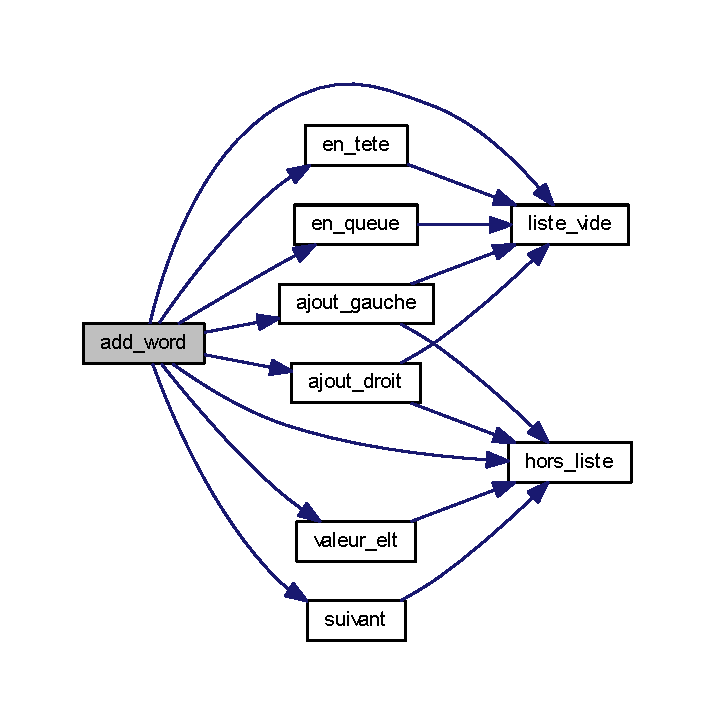
\includegraphics[width=343pt]{d3/df5/ruzzle_8c_ab7e43a2c2790bc312915ec6654ec59ec_cgraph}
\end{center}
\end{figure}


\hypertarget{ruzzle_8c_a718478def452ab5bca4b1a3bc8393c57}{}\index{ruzzle.\+c@{ruzzle.\+c}!create\+\_\+new\+\_\+dico@{create\+\_\+new\+\_\+dico}}
\index{create\+\_\+new\+\_\+dico@{create\+\_\+new\+\_\+dico}!ruzzle.\+c@{ruzzle.\+c}}
\subsubsection[{create\+\_\+new\+\_\+dico(cell ruzzle[N][N], F\+I\+L\+E $\ast$dico)}]{\setlength{\rightskip}{0pt plus 5cm}int create\+\_\+new\+\_\+dico (
\begin{DoxyParamCaption}
\item[{{\bf cell}}]{ruzzle\mbox{[}\+N\mbox{]}\mbox{[}\+N\mbox{]}, }
\item[{F\+I\+L\+E $\ast$}]{dico}
\end{DoxyParamCaption}
)}\label{ruzzle_8c_a718478def452ab5bca4b1a3bc8393c57}


Crée un dictionaire élagué 


\begin{DoxyParams}{Paramètres}
{\em cell} & ruzzle\mbox{[}N\mbox{]}\mbox{[}N\mbox{]} \+: matrice du ruzzle \\
\hline
{\em F\+I\+L\+E} & $\ast$ dico \+: dictionnaire complet \\
\hline
\end{DoxyParams}
\begin{DoxyReturn}{Renvoie}
renvoie toujours 0 (pourait être amélioré en renvoiyant un code d\textquotesingle{}erreur)
\end{DoxyReturn}
Crée un nouveau dictionnaire appelé nexdico.\+txt qui ne contiend que les mot dont les lettres sont présentes dans la grille. Cette fonction permet de réduire la taille du fichier parcouru de 3.\+6\+Mo à environ 800\+Ko. 

Définition à la ligne 101 du fichier ruzzle.\+c.

\hypertarget{ruzzle_8c_ad285e4b1ee303ca9809b0aeb31d62685}{}\index{ruzzle.\+c@{ruzzle.\+c}!find\+\_\+letter@{find\+\_\+letter}}
\index{find\+\_\+letter@{find\+\_\+letter}!ruzzle.\+c@{ruzzle.\+c}}
\subsubsection[{find\+\_\+letter(char c, coord $\ast$pos, cell ruzzle[N][N])}]{\setlength{\rightskip}{0pt plus 5cm}bool find\+\_\+letter (
\begin{DoxyParamCaption}
\item[{char}]{c, }
\item[{{\bf coord} $\ast$}]{pos, }
\item[{{\bf cell}}]{ruzzle\mbox{[}\+N\mbox{]}\mbox{[}\+N\mbox{]}}
\end{DoxyParamCaption}
)}\label{ruzzle_8c_ad285e4b1ee303ca9809b0aeb31d62685}


Trouve la lettre autour de la position passée en paramètre. 


\begin{DoxyParams}{Paramètres}
{\em char} & c charactère recherché \\
\hline
{\em coord} & $\ast$ pos position autour de laquel chercher \\
\hline
{\em cell} & ruzzle\mbox{[}N\mbox{]}\mbox{[}N\mbox{]} \+: grille du ruzzle \\
\hline
\end{DoxyParams}
\begin{DoxyReturn}{Renvoie}
retourne true si la lettre à été trouvé, false sinon. 
\end{DoxyReturn}


Définition à la ligne 159 du fichier ruzzle.\+c.

\hypertarget{ruzzle_8c_a3c8d832e7a79666902bf858650d6ef33}{}\index{ruzzle.\+c@{ruzzle.\+c}!find\+\_\+word@{find\+\_\+word}}
\index{find\+\_\+word@{find\+\_\+word}!ruzzle.\+c@{ruzzle.\+c}}
\subsubsection[{find\+\_\+word(cell ruzzle[N][N], char mot[])}]{\setlength{\rightskip}{0pt plus 5cm}void find\+\_\+word (
\begin{DoxyParamCaption}
\item[{{\bf cell}}]{ruzzle\mbox{[}\+N\mbox{]}\mbox{[}\+N\mbox{]}, }
\item[{char}]{mot\mbox{[}$\,$\mbox{]}}
\end{DoxyParamCaption}
)}\label{ruzzle_8c_a3c8d832e7a79666902bf858650d6ef33}


Cherche un mot dans la grille. 


\begin{DoxyParams}{Paramètres}
{\em cell} & ruzzle\mbox{[}N\mbox{]}\mbox{[}N\mbox{]} grille du ruzzle \\
\hline
{\em char} & mot\mbox{[}\mbox{]} un mot du dictionnaire à chercher dans la grille\\
\hline
\end{DoxyParams}
find\+\_\+word prend en paramètre la grille du ruzzle et un mot, cherche le mot a l\textquotesingle{}aide d\textquotesingle{}autre fonction et l\textquotesingle{}inscrit dans la liste des solution avec son score. 

Définition à la ligne 285 du fichier ruzzle.\+c.



Voici le graphe d\textquotesingle{}appel pour cette fonction \+:
\nopagebreak
\begin{figure}[H]
\begin{center}
\leavevmode
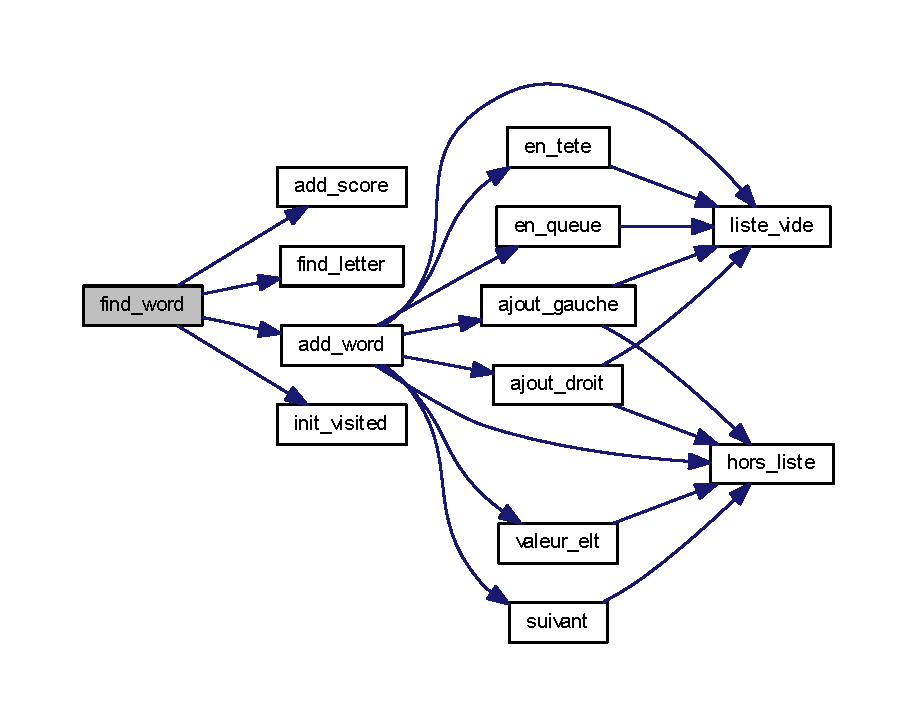
\includegraphics[width=350pt]{d3/df5/ruzzle_8c_a3c8d832e7a79666902bf858650d6ef33_cgraph}
\end{center}
\end{figure}


\hypertarget{ruzzle_8c_a17b31853d3aa79a67d0c25a3ae68a89a}{}\index{ruzzle.\+c@{ruzzle.\+c}!init@{init}}
\index{init@{init}!ruzzle.\+c@{ruzzle.\+c}}
\subsubsection[{init(char entree[], cell sortie[N][N], F\+I\+L\+E $\ast$dico, F\+I\+L\+E $\ast$output)}]{\setlength{\rightskip}{0pt plus 5cm}int init (
\begin{DoxyParamCaption}
\item[{char}]{entree\mbox{[}$\,$\mbox{]}, }
\item[{{\bf cell}}]{sortie\mbox{[}\+N\mbox{]}\mbox{[}\+N\mbox{]}, }
\item[{F\+I\+L\+E $\ast$}]{dico, }
\item[{F\+I\+L\+E $\ast$}]{output}
\end{DoxyParamCaption}
)}\label{ruzzle_8c_a17b31853d3aa79a67d0c25a3ae68a89a}


Fonction d\textquotesingle{}initialisation globale. 


\begin{DoxyParams}{Paramètres}
{\em char} & entree\mbox{[}\mbox{]} les lettres de la grille du ruzzle. \\
\hline
{\em cell} & sortie\mbox{[}N\mbox{]}\mbox{[}N\mbox{]} la transformé en tableau de entree\mbox{[}\mbox{]}. \\
\hline
{\em F\+I\+L\+E} & $\ast$ dico le dictionnaire complet \\
\hline
{\em F\+I\+L\+E} & $\ast$ output le fichier où seront placé les mot possible.\\
\hline
\end{DoxyParams}
\begin{DoxyReturn}{Renvoie}
Renvoit un code d\textquotesingle{}erreur si besoin, 0 sinon.
\end{DoxyReturn}
Initialise la grille avec les lettre passées en paramètre et verifie que les fichiers soient accessibles. 

Définition à la ligne 29 du fichier ruzzle.\+c.

\hypertarget{ruzzle_8c_ac56429d3c5f2133304acb4b6e461cc1b}{}\index{ruzzle.\+c@{ruzzle.\+c}!init\+\_\+visited@{init\+\_\+visited}}
\index{init\+\_\+visited@{init\+\_\+visited}!ruzzle.\+c@{ruzzle.\+c}}
\subsubsection[{init\+\_\+visited(cell ruzzle[N][N])}]{\setlength{\rightskip}{0pt plus 5cm}void init\+\_\+visited (
\begin{DoxyParamCaption}
\item[{{\bf cell}}]{ruzzle\mbox{[}\+N\mbox{]}\mbox{[}\+N\mbox{]}}
\end{DoxyParamCaption}
)}\label{ruzzle_8c_ac56429d3c5f2133304acb4b6e461cc1b}


Réinitialise le statut visité de chaque case. 


\begin{DoxyParams}{Paramètres}
{\em cell} & ruzzle\mbox{[}N\mbox{]}\mbox{[}N\mbox{]} grille du ruzzle\\
\hline
\end{DoxyParams}
init\+\_\+visit prend la grille du ruzzle en paramètre et réinitialise le booléen qui indique le passage ou non sur une case en le passant à false. 

Définition à la ligne 261 du fichier ruzzle.\+c.

\hypertarget{ruzzle_8c_ad9429c78019005dc6e8e62a30166c64b}{}\index{ruzzle.\+c@{ruzzle.\+c}!print\+\_\+list@{print\+\_\+list}}
\index{print\+\_\+list@{print\+\_\+list}!ruzzle.\+c@{ruzzle.\+c}}
\subsubsection[{print\+\_\+list()}]{\setlength{\rightskip}{0pt plus 5cm}void print\+\_\+list (
\begin{DoxyParamCaption}
{}
\end{DoxyParamCaption}
)}\label{ruzzle_8c_ad9429c78019005dc6e8e62a30166c64b}


Enregiste la liste des mots possible dans un fichier externe. 



Définition à la ligne 337 du fichier ruzzle.\+c.



Voici le graphe d\textquotesingle{}appel pour cette fonction \+:
\nopagebreak
\begin{figure}[H]
\begin{center}
\leavevmode
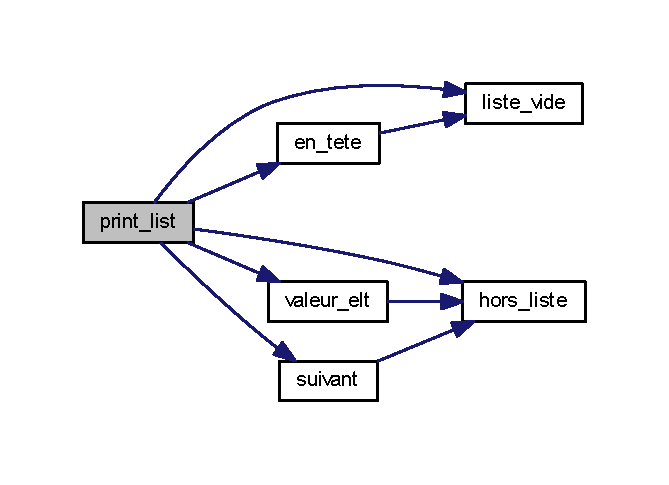
\includegraphics[width=321pt]{d3/df5/ruzzle_8c_ad9429c78019005dc6e8e62a30166c64b_cgraph}
\end{center}
\end{figure}



\hypertarget{ruzzle_8h}{}\section{Référence du fichier ruzzle.\+h}
\label{ruzzle_8h}\index{ruzzle.\+h@{ruzzle.\+h}}
{\ttfamily \#include $<$stdio.\+h$>$}\\*
{\ttfamily \#include $<$stdbool.\+h$>$}\\*
Graphe des dépendances par inclusion de ruzzle.\+h\+:
\nopagebreak
\begin{figure}[H]
\begin{center}
\leavevmode
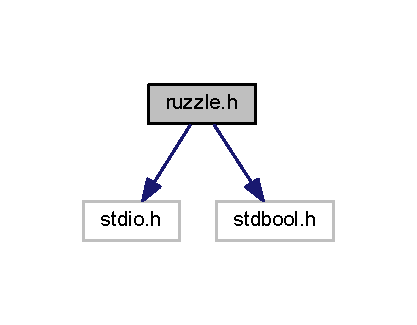
\includegraphics[width=200pt]{df/ddf/ruzzle_8h__incl}
\end{center}
\end{figure}
Ce graphe montre quels fichiers incluent directement ou indirectement ce fichier \+:
\nopagebreak
\begin{figure}[H]
\begin{center}
\leavevmode
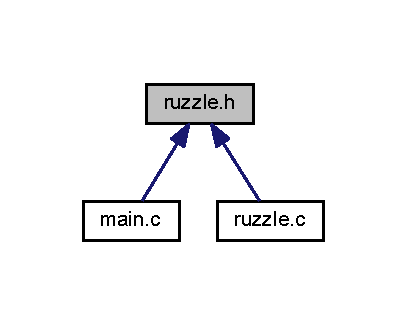
\includegraphics[width=196pt]{d5/d10/ruzzle_8h__dep__incl}
\end{center}
\end{figure}
\subsection*{Structures de données}
\begin{DoxyCompactItemize}
\item 
struct \hyperlink{structcell}{cell}
\begin{DoxyCompactList}\small\item\em Défini une case de la grille, l\textquotesingle{}élément \textquotesingle{}visited\textquotesingle{} est utilisé lors de la recherche de mot. \end{DoxyCompactList}\item 
struct \hyperlink{structcoord}{coord}
\begin{DoxyCompactList}\small\item\em Défini des coordonnée d\textquotesingle{}une case de la grille. \end{DoxyCompactList}\item 
struct \hyperlink{structt__score}{t\+\_\+score}
\begin{DoxyCompactList}\small\item\em défini le score du mot que l\textquotesingle{}on est en train de chercher. \end{DoxyCompactList}\end{DoxyCompactItemize}
\subsection*{Macros}
\begin{DoxyCompactItemize}
\item 
\#define \hyperlink{ruzzle_8h_a0240ac851181b84ac374872dc5434ee4}{N}~4
\end{DoxyCompactItemize}
\subsection*{Énumérations}
\begin{DoxyCompactItemize}
\item 
enum \hyperlink{ruzzle_8h_af98046282a9e785a234a2ea7b10681f2}{bonus\+Enum} \{ \\*
\hyperlink{ruzzle_8h_af98046282a9e785a234a2ea7b10681f2ab7e4e0120a041dbe6528b050c04269e0}{none} = 1, 
\hyperlink{ruzzle_8h_af98046282a9e785a234a2ea7b10681f2ab53f15e4bbe81ad687b79e42ca75244e}{double\+L} = 2, 
\hyperlink{ruzzle_8h_af98046282a9e785a234a2ea7b10681f2a471cc885602be95c5808f4b6456cb94e}{triple\+L} = 3, 
\hyperlink{ruzzle_8h_af98046282a9e785a234a2ea7b10681f2a600130c1478bc563fb6b2e92e07a3aed}{double\+M} = 4, 
\\*
\hyperlink{ruzzle_8h_af98046282a9e785a234a2ea7b10681f2a49f2ded5d4ef00d67a76019ae3375a9e}{triple\+M} = 6
 \}\begin{DoxyCompactList}\small\item\em Énumération des différents bonus possibles. \end{DoxyCompactList}
\end{DoxyCompactItemize}
\subsection*{Fonctions}
\begin{DoxyCompactItemize}
\item 
int \hyperlink{ruzzle_8h_acb1b1746387e6aa6adcaac13a060b15a}{init} (char\mbox{[}$\,$\mbox{]}, \hyperlink{structcell}{cell}\mbox{[}\hyperlink{ruzzle_8h_a0240ac851181b84ac374872dc5434ee4}{N}\mbox{]}\mbox{[}\hyperlink{ruzzle_8h_a0240ac851181b84ac374872dc5434ee4}{N}\mbox{]}, F\+I\+L\+E $\ast$, F\+I\+L\+E $\ast$)
\begin{DoxyCompactList}\small\item\em Fonction d\textquotesingle{}initialisation globale. \end{DoxyCompactList}\item 
int \hyperlink{ruzzle_8h_a08a07b0e604daf115ce1091c0614da22}{create\+\_\+new\+\_\+dico} (\hyperlink{structcell}{cell}\mbox{[}\hyperlink{ruzzle_8h_a0240ac851181b84ac374872dc5434ee4}{N}\mbox{]}\mbox{[}\hyperlink{ruzzle_8h_a0240ac851181b84ac374872dc5434ee4}{N}\mbox{]}, F\+I\+L\+E $\ast$)
\begin{DoxyCompactList}\small\item\em Crée un dictionaire élagué \end{DoxyCompactList}\item 
bool \hyperlink{ruzzle_8h_ad590be2d37e435837a2ea6137c27c05a}{find\+\_\+letter} (char, \hyperlink{structcoord}{coord} $\ast$, \hyperlink{structcell}{cell}\mbox{[}\hyperlink{ruzzle_8h_a0240ac851181b84ac374872dc5434ee4}{N}\mbox{]}\mbox{[}\hyperlink{ruzzle_8h_a0240ac851181b84ac374872dc5434ee4}{N}\mbox{]})
\begin{DoxyCompactList}\small\item\em Trouve la lettre autour de la position passée en paramètre. \end{DoxyCompactList}\item 
void \hyperlink{ruzzle_8h_a2e0f456b7e11b42478bd1062c4aa7625}{ajouter\+\_\+mot} (char $\ast$, int)
\item 
void \hyperlink{ruzzle_8h_a8b51c038f96e507ab15d6ef3edfa3210}{ajouter\+\_\+score} (\hyperlink{structcell}{cell}\mbox{[}\hyperlink{ruzzle_8h_a0240ac851181b84ac374872dc5434ee4}{N}\mbox{]}\mbox{[}\hyperlink{ruzzle_8h_a0240ac851181b84ac374872dc5434ee4}{N}\mbox{]}, \hyperlink{structcoord}{coord}, \hyperlink{structt__score}{t\+\_\+score} $\ast$)
\item 
void \hyperlink{ruzzle_8h_a605e27e92e36decc89320b12d494e6d8}{init\+\_\+visited} (\hyperlink{structcell}{cell}\mbox{[}\hyperlink{ruzzle_8h_a0240ac851181b84ac374872dc5434ee4}{N}\mbox{]}\mbox{[}\hyperlink{ruzzle_8h_a0240ac851181b84ac374872dc5434ee4}{N}\mbox{]})
\begin{DoxyCompactList}\small\item\em Réinitialise le statut visité de chaque case. \end{DoxyCompactList}\item 
void \hyperlink{ruzzle_8h_a6668f0d4ced5473df624a0cccb0dcf6c}{find\+\_\+word} (\hyperlink{structcell}{cell}\mbox{[}\hyperlink{ruzzle_8h_a0240ac851181b84ac374872dc5434ee4}{N}\mbox{]}\mbox{[}\hyperlink{ruzzle_8h_a0240ac851181b84ac374872dc5434ee4}{N}\mbox{]}, char\mbox{[}$\,$\mbox{]})
\begin{DoxyCompactList}\small\item\em Cherche un mot dans la grille. \end{DoxyCompactList}\item 
void \hyperlink{ruzzle_8h_ad9429c78019005dc6e8e62a30166c64b}{print\+\_\+list} ()
\begin{DoxyCompactList}\small\item\em Enregiste la liste des mots possible dans un fichier externe. \end{DoxyCompactList}\end{DoxyCompactItemize}


\subsection{Documentation des macros}
\hypertarget{ruzzle_8h_a0240ac851181b84ac374872dc5434ee4}{}\index{ruzzle.\+h@{ruzzle.\+h}!N@{N}}
\index{N@{N}!ruzzle.\+h@{ruzzle.\+h}}
\subsubsection[{N}]{\setlength{\rightskip}{0pt plus 5cm}\#define N~4}\label{ruzzle_8h_a0240ac851181b84ac374872dc5434ee4}


Définition à la ligne 4 du fichier ruzzle.\+h.



\subsection{Documentation du type de l\textquotesingle{}énumération}
\hypertarget{ruzzle_8h_af98046282a9e785a234a2ea7b10681f2}{}\index{ruzzle.\+h@{ruzzle.\+h}!bonus\+Enum@{bonus\+Enum}}
\index{bonus\+Enum@{bonus\+Enum}!ruzzle.\+h@{ruzzle.\+h}}
\subsubsection[{bonus\+Enum}]{\setlength{\rightskip}{0pt plus 5cm}enum {\bf bonus\+Enum}}\label{ruzzle_8h_af98046282a9e785a234a2ea7b10681f2}


Énumération des différents bonus possibles. 

\begin{Desc}
\item[Valeurs énumérées]\par
\begin{description}
\index{none@{none}!ruzzle.\+h@{ruzzle.\+h}}\index{ruzzle.\+h@{ruzzle.\+h}!none@{none}}\item[{\em 
\hypertarget{ruzzle_8h_af98046282a9e785a234a2ea7b10681f2ab7e4e0120a041dbe6528b050c04269e0}{}none\label{ruzzle_8h_af98046282a9e785a234a2ea7b10681f2ab7e4e0120a041dbe6528b050c04269e0}
}]\index{double\+L@{double\+L}!ruzzle.\+h@{ruzzle.\+h}}\index{ruzzle.\+h@{ruzzle.\+h}!double\+L@{double\+L}}\item[{\em 
\hypertarget{ruzzle_8h_af98046282a9e785a234a2ea7b10681f2ab53f15e4bbe81ad687b79e42ca75244e}{}double\+L\label{ruzzle_8h_af98046282a9e785a234a2ea7b10681f2ab53f15e4bbe81ad687b79e42ca75244e}
}]\index{triple\+L@{triple\+L}!ruzzle.\+h@{ruzzle.\+h}}\index{ruzzle.\+h@{ruzzle.\+h}!triple\+L@{triple\+L}}\item[{\em 
\hypertarget{ruzzle_8h_af98046282a9e785a234a2ea7b10681f2a471cc885602be95c5808f4b6456cb94e}{}triple\+L\label{ruzzle_8h_af98046282a9e785a234a2ea7b10681f2a471cc885602be95c5808f4b6456cb94e}
}]\index{double\+M@{double\+M}!ruzzle.\+h@{ruzzle.\+h}}\index{ruzzle.\+h@{ruzzle.\+h}!double\+M@{double\+M}}\item[{\em 
\hypertarget{ruzzle_8h_af98046282a9e785a234a2ea7b10681f2a600130c1478bc563fb6b2e92e07a3aed}{}double\+M\label{ruzzle_8h_af98046282a9e785a234a2ea7b10681f2a600130c1478bc563fb6b2e92e07a3aed}
}]\index{triple\+M@{triple\+M}!ruzzle.\+h@{ruzzle.\+h}}\index{ruzzle.\+h@{ruzzle.\+h}!triple\+M@{triple\+M}}\item[{\em 
\hypertarget{ruzzle_8h_af98046282a9e785a234a2ea7b10681f2a49f2ded5d4ef00d67a76019ae3375a9e}{}triple\+M\label{ruzzle_8h_af98046282a9e785a234a2ea7b10681f2a49f2ded5d4ef00d67a76019ae3375a9e}
}]\end{description}
\end{Desc}


Définition à la ligne 9 du fichier ruzzle.\+h.



\subsection{Documentation des fonctions}
\hypertarget{ruzzle_8h_a2e0f456b7e11b42478bd1062c4aa7625}{}\index{ruzzle.\+h@{ruzzle.\+h}!ajouter\+\_\+mot@{ajouter\+\_\+mot}}
\index{ajouter\+\_\+mot@{ajouter\+\_\+mot}!ruzzle.\+h@{ruzzle.\+h}}
\subsubsection[{ajouter\+\_\+mot(char $\ast$, int)}]{\setlength{\rightskip}{0pt plus 5cm}void ajouter\+\_\+mot (
\begin{DoxyParamCaption}
\item[{char $\ast$}]{, }
\item[{int}]{}
\end{DoxyParamCaption}
)}\label{ruzzle_8h_a2e0f456b7e11b42478bd1062c4aa7625}
\hypertarget{ruzzle_8h_a8b51c038f96e507ab15d6ef3edfa3210}{}\index{ruzzle.\+h@{ruzzle.\+h}!ajouter\+\_\+score@{ajouter\+\_\+score}}
\index{ajouter\+\_\+score@{ajouter\+\_\+score}!ruzzle.\+h@{ruzzle.\+h}}
\subsubsection[{ajouter\+\_\+score(cell[N][N], coord, t\+\_\+score $\ast$)}]{\setlength{\rightskip}{0pt plus 5cm}void ajouter\+\_\+score (
\begin{DoxyParamCaption}
\item[{{\bf cell}}]{\mbox{[}\+N\mbox{]}\mbox{[}\+N\mbox{]}, }
\item[{{\bf coord}}]{, }
\item[{{\bf t\+\_\+score} $\ast$}]{}
\end{DoxyParamCaption}
)}\label{ruzzle_8h_a8b51c038f96e507ab15d6ef3edfa3210}
\hypertarget{ruzzle_8h_a08a07b0e604daf115ce1091c0614da22}{}\index{ruzzle.\+h@{ruzzle.\+h}!create\+\_\+new\+\_\+dico@{create\+\_\+new\+\_\+dico}}
\index{create\+\_\+new\+\_\+dico@{create\+\_\+new\+\_\+dico}!ruzzle.\+h@{ruzzle.\+h}}
\subsubsection[{create\+\_\+new\+\_\+dico(cell[N][N], F\+I\+L\+E $\ast$)}]{\setlength{\rightskip}{0pt plus 5cm}int create\+\_\+new\+\_\+dico (
\begin{DoxyParamCaption}
\item[{{\bf cell}}]{ruzzle\mbox{[}\+N\mbox{]}\mbox{[}\+N\mbox{]}, }
\item[{F\+I\+L\+E $\ast$}]{dico}
\end{DoxyParamCaption}
)}\label{ruzzle_8h_a08a07b0e604daf115ce1091c0614da22}


Crée un dictionaire élagué 


\begin{DoxyParams}{Paramètres}
{\em cell} & ruzzle\mbox{[}N\mbox{]}\mbox{[}N\mbox{]} \+: matrice du ruzzle \\
\hline
{\em F\+I\+L\+E} & $\ast$ dico \+: dictionnaire complet \\
\hline
\end{DoxyParams}
\begin{DoxyReturn}{Renvoie}
renvoie toujours 0 (pourait être amélioré en renvoiyant un code d\textquotesingle{}erreur)
\end{DoxyReturn}
Crée un nouveau dictionnaire appelé nexdico.\+txt qui ne contiend que les mot dont les lettres sont présentes dans la grille. Cette fonction permet de réduire la taille du fichier parcouru de 3.\+6\+Mo à environ 800\+Ko. 

Définition à la ligne 101 du fichier ruzzle.\+c.

\hypertarget{ruzzle_8h_ad590be2d37e435837a2ea6137c27c05a}{}\index{ruzzle.\+h@{ruzzle.\+h}!find\+\_\+letter@{find\+\_\+letter}}
\index{find\+\_\+letter@{find\+\_\+letter}!ruzzle.\+h@{ruzzle.\+h}}
\subsubsection[{find\+\_\+letter(char, coord $\ast$, cell[N][N])}]{\setlength{\rightskip}{0pt plus 5cm}bool find\+\_\+letter (
\begin{DoxyParamCaption}
\item[{char}]{c, }
\item[{{\bf coord} $\ast$}]{pos, }
\item[{{\bf cell}}]{ruzzle\mbox{[}\+N\mbox{]}\mbox{[}\+N\mbox{]}}
\end{DoxyParamCaption}
)}\label{ruzzle_8h_ad590be2d37e435837a2ea6137c27c05a}


Trouve la lettre autour de la position passée en paramètre. 


\begin{DoxyParams}{Paramètres}
{\em char} & c charactère recherché \\
\hline
{\em coord} & $\ast$ pos position autour de laquel chercher \\
\hline
{\em cell} & ruzzle\mbox{[}N\mbox{]}\mbox{[}N\mbox{]} \+: grille du ruzzle \\
\hline
\end{DoxyParams}
\begin{DoxyReturn}{Renvoie}
retourne true si la lettre à été trouvé, false sinon. 
\end{DoxyReturn}


Définition à la ligne 159 du fichier ruzzle.\+c.

\hypertarget{ruzzle_8h_a6668f0d4ced5473df624a0cccb0dcf6c}{}\index{ruzzle.\+h@{ruzzle.\+h}!find\+\_\+word@{find\+\_\+word}}
\index{find\+\_\+word@{find\+\_\+word}!ruzzle.\+h@{ruzzle.\+h}}
\subsubsection[{find\+\_\+word(cell[N][N], char[])}]{\setlength{\rightskip}{0pt plus 5cm}void find\+\_\+word (
\begin{DoxyParamCaption}
\item[{{\bf cell}}]{ruzzle\mbox{[}\+N\mbox{]}\mbox{[}\+N\mbox{]}, }
\item[{char}]{mot\mbox{[}$\,$\mbox{]}}
\end{DoxyParamCaption}
)}\label{ruzzle_8h_a6668f0d4ced5473df624a0cccb0dcf6c}


Cherche un mot dans la grille. 


\begin{DoxyParams}{Paramètres}
{\em cell} & ruzzle\mbox{[}N\mbox{]}\mbox{[}N\mbox{]} grille du ruzzle \\
\hline
{\em char} & mot\mbox{[}\mbox{]} un mot du dictionnaire à chercher dans la grille\\
\hline
\end{DoxyParams}
find\+\_\+word prend en paramètre la grille du ruzzle et un mot, cherche le mot a l\textquotesingle{}aide d\textquotesingle{}autre fonction et l\textquotesingle{}inscrit dans la liste des solution avec son score. 

Définition à la ligne 285 du fichier ruzzle.\+c.



Voici le graphe d\textquotesingle{}appel pour cette fonction \+:
\nopagebreak
\begin{figure}[H]
\begin{center}
\leavevmode
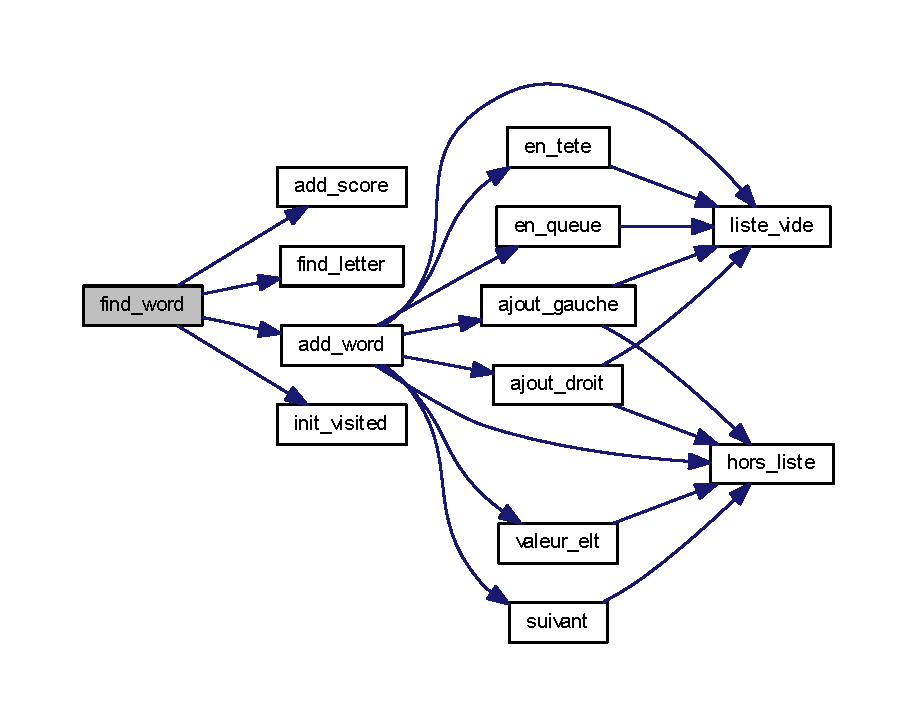
\includegraphics[width=350pt]{df/d02/ruzzle_8h_a6668f0d4ced5473df624a0cccb0dcf6c_cgraph}
\end{center}
\end{figure}


\hypertarget{ruzzle_8h_acb1b1746387e6aa6adcaac13a060b15a}{}\index{ruzzle.\+h@{ruzzle.\+h}!init@{init}}
\index{init@{init}!ruzzle.\+h@{ruzzle.\+h}}
\subsubsection[{init(char[], cell[N][N], F\+I\+L\+E $\ast$, F\+I\+L\+E $\ast$)}]{\setlength{\rightskip}{0pt plus 5cm}int init (
\begin{DoxyParamCaption}
\item[{char}]{entree\mbox{[}$\,$\mbox{]}, }
\item[{{\bf cell}}]{sortie\mbox{[}\+N\mbox{]}\mbox{[}\+N\mbox{]}, }
\item[{F\+I\+L\+E $\ast$}]{dico, }
\item[{F\+I\+L\+E $\ast$}]{output}
\end{DoxyParamCaption}
)}\label{ruzzle_8h_acb1b1746387e6aa6adcaac13a060b15a}


Fonction d\textquotesingle{}initialisation globale. 


\begin{DoxyParams}{Paramètres}
{\em char} & entree\mbox{[}\mbox{]} les lettres de la grille du ruzzle. \\
\hline
{\em cell} & sortie\mbox{[}N\mbox{]}\mbox{[}N\mbox{]} la transformé en tableau de entree\mbox{[}\mbox{]}. \\
\hline
{\em F\+I\+L\+E} & $\ast$ dico le dictionnaire complet \\
\hline
{\em F\+I\+L\+E} & $\ast$ output le fichier où seront placé les mot possible.\\
\hline
\end{DoxyParams}
\begin{DoxyReturn}{Renvoie}
Renvoit un code d\textquotesingle{}erreur si besoin, 0 sinon.
\end{DoxyReturn}
Initialise la grille avec les lettre passées en paramètre et verifie que les fichiers soient accessibles. 

Définition à la ligne 29 du fichier ruzzle.\+c.

\hypertarget{ruzzle_8h_a605e27e92e36decc89320b12d494e6d8}{}\index{ruzzle.\+h@{ruzzle.\+h}!init\+\_\+visited@{init\+\_\+visited}}
\index{init\+\_\+visited@{init\+\_\+visited}!ruzzle.\+h@{ruzzle.\+h}}
\subsubsection[{init\+\_\+visited(cell[N][N])}]{\setlength{\rightskip}{0pt plus 5cm}void init\+\_\+visited (
\begin{DoxyParamCaption}
\item[{{\bf cell}}]{ruzzle\mbox{[}\+N\mbox{]}\mbox{[}\+N\mbox{]}}
\end{DoxyParamCaption}
)}\label{ruzzle_8h_a605e27e92e36decc89320b12d494e6d8}


Réinitialise le statut visité de chaque case. 


\begin{DoxyParams}{Paramètres}
{\em cell} & ruzzle\mbox{[}N\mbox{]}\mbox{[}N\mbox{]} grille du ruzzle\\
\hline
\end{DoxyParams}
init\+\_\+visit prend la grille du ruzzle en paramètre et réinitialise le booléen qui indique le passage ou non sur une case en le passant à false. 

Définition à la ligne 261 du fichier ruzzle.\+c.

\hypertarget{ruzzle_8h_ad9429c78019005dc6e8e62a30166c64b}{}\index{ruzzle.\+h@{ruzzle.\+h}!print\+\_\+list@{print\+\_\+list}}
\index{print\+\_\+list@{print\+\_\+list}!ruzzle.\+h@{ruzzle.\+h}}
\subsubsection[{print\+\_\+list()}]{\setlength{\rightskip}{0pt plus 5cm}void print\+\_\+list (
\begin{DoxyParamCaption}
{}
\end{DoxyParamCaption}
)}\label{ruzzle_8h_ad9429c78019005dc6e8e62a30166c64b}


Enregiste la liste des mots possible dans un fichier externe. 



Définition à la ligne 337 du fichier ruzzle.\+c.



Voici le graphe d\textquotesingle{}appel pour cette fonction \+:
\nopagebreak
\begin{figure}[H]
\begin{center}
\leavevmode
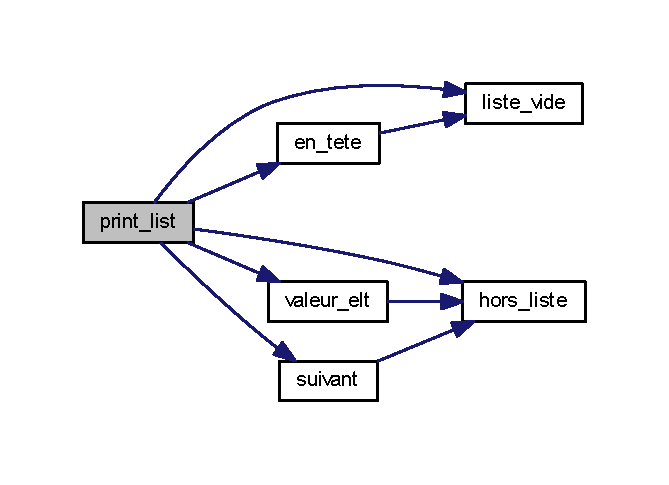
\includegraphics[width=321pt]{df/d02/ruzzle_8h_ad9429c78019005dc6e8e62a30166c64b_cgraph}
\end{center}
\end{figure}



%--- End generated contents ---

% Index
\backmatter
\newpage
\phantomsection
\clearemptydoublepage
\addcontentsline{toc}{chapter}{Index}
\printindex

\end{document}
